\documentclass[pdftex,12pt,a4paper]{report}

\usepackage[utf8]{inputenc}
\usepackage[T1]{fontenc}
\usepackage[francais]{babel}
\usepackage{setspace}
\usepackage[top=2.5cm,bottom=2.5cm,right=3cm,left=3cm]{geometry}
\usepackage{parskip}

\usepackage{hyperref}
\usepackage{color}

\usepackage{calc}
\usepackage{pseudocode}

\usepackage[pdftex]{graphicx}
\usepackage{float}
\usepackage{fancybox}

\usepackage{caption}
\captionsetup{figurewithin=none}  
\captionsetup{tablewithin=none}

\AddThinSpaceBeforeFootnotes

\FrenchFootnotes

\newcommand{\HRule}{\rule{\linewidth}{1mm}}

\setlength{\parskip}{1mm}

\begin{document}
\begin{spacing}{1.2}

%Thème utilisé sur http://en.wikibooks.org/wiki/LaTeX/Title_Creation
\begin{titlepage}
\begin{center}


\includegraphics[scale=0.25]{img/logo-lille1.jpg}\\[2.5cm]

%\textsc{\LARGE Universite Lille1}\\[1cm]

\textsc{\Large \bfseries Rapport de stage - Licence informatique}\\[0.5cm]

% Title
\HRule \\[0.5cm]
{ \Large \bfseries Visualisation des clones V(D)J en fonction des distances d'édition, et suivi de la Leucémie Aigue Lymphoblastique \\[0.5cm]}
\HRule \\[0.5cm]

\textsc{\large Laboratoire d'Informatique Fondamentale de Lille - Équipe ``Bonsai''}\\[2cm]

% Author and supervisor
\begin{minipage}{0.4\textwidth}
\begin{flushleft} \large
\emph{\bfseries Auteur:}\\
Antonin \textsc{Carette}
\end{flushleft}
\end{minipage}
\begin{minipage}{0.4\textwidth}
\begin{flushright} \large
\emph{\bfseries Tuteur Entreprise:} \\
Dr.~Mathieu \textsc{Giraud}\\[0.2cm]
\emph{\bfseries Tuteur Universitaire:} \\
Dr.~Samy \textsc{Meftali}
\end{flushright}
\end{minipage}

\vfill

\begin{figure}[H]
    \begin{minipage}[t]{8cm}
        \centering
	
\includegraphics[scale=0.15]{img/logo-lifl.png}
    \end{minipage}
    \begin{minipage}[t]{8cm}
        \centering
        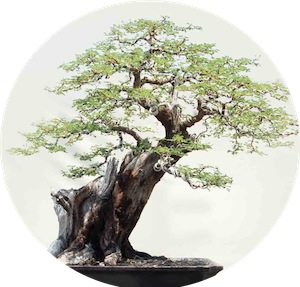
\includegraphics[scale=1]{img/bonsai-rond.jpg}
    \end{minipage}
\end{figure}

\vfill

% Bottom of the page
{\large Compilé le \today}

\end{center}
\end{titlepage}

\tableofcontents

\chapter*{Introduction}

\addcontentsline{toc}{chapter}{Introduction} 

\section{Remerciements}
Je remercie tout d'abord mon tuteur d'Université: \textbf{Samy Meftali}, ainsi que mon tuteur en entreprise: \textbf{Mathieu Giraud}, pour toute l'attention donnée quant au travail sur le projet, ainsi que sur ce rapport.
\newline
Je remercie ensuite l'équipe \textit{Bonsai} ainsi que les membres du projet \textit{Vidjil}, pour leur accueil ainsi que leur soutien, recueillis durant les 3 mois de stage.
\newline
Enfin, je tiens à remercier mes collèges du bureau 235: \textbf{Yoann Dufresne} et M. \textbf{Christophe Vrolland}.

\section{Présentation de l'entreprise et de l'équipe}

\subsection{Le \textit{LIFL}}
Le \textit{LIFL} (Laboratoire d'Informatique Fondamentale de Lille) est un laboratoire Français fondé en 1983, présent sur le campus de l'Université Lille1, rattaché à l'Institut des Sciences de l'Information et de leurs Interactions (\textit{INS2I}) du \textit{CNRS} (Centre National de la Recherche Scientifique).
\newline
Il est maintenant dirigé par \textbf{Sophie Tison} comprend 10 équipes-projets et équipes du centre de recherche \textit{INRIA} Lille - Nord Europe (Institut national de recherche en informatique et en automatique), de recherches diverses et variées (axe Mathématique, Réalité Virtuelle, BioInformatique, Sécurité et Réseau, Systèmes Multi-agents, etc...); aujourd'hui, plus de 300 personnes y travaillent (enseignants-chercheurs, ingénieurs, techniciens, administratifs et doctorants).

\subsection{L'équipe \textit{Bonsai}}
\textit{Bonsai} est une équipe du \textit{LIFL}, auparavant nommée \textit{Sequoia}.
Cette jeune équipe dépend du \textit{LIFL}, de l'\textit{INRIA} ainsi que du \textit{CNRS}, et est dirigée par \textbf{Hélène Touzet}.
\newline
Les travaux des membres de l'équipe (on en compte actuellement 22) sont tous réunis dans un seul grand domaine: la Biologie.
En effet, l'équipe \textit{Bonsai} est très réputée dans la bio-informatique; on dénombre aujourd'hui plus de 30 applications/logiciels utilisables gratuitement\footnote{Ces logiciels sont consultables sur le site internet de l'équipe: \url{http://bioinfo.lifl.fr}}, créés par les membres de l'équipe.
\newline
Cette équipe m'a donc accueillie pour mon stage de fin de licence, s'étant déroulé du 1er Avril au 30 Juin 2014, mes encadrants étant \textbf{Mathieu Giraud} (mon tuteur en entreprise), \textbf{Mikaël Salson} ainsi que \textbf{Marc Duez}, ingénieur du projet \textit{Vidjil}.


\chapter{Contexte du stage et objectifs}

\section{La Leucémie Aigüe Lymphoblastique}

Chaque Humain et Vertébré détient un système de recombinaison de l'ADN (que l'on appelle \textbf{recombinaison V(D)J}\footnote{Phénomène biologique impliquant des processus par lesquels une molécule d'ADN (ou d'ARN) est coupée, puis jointe à une autre.}), mécanisme permettant de créer une grande diversité de récepteurs d'antigènes (nécessaires à la reconnaissance de corps étrangers), et donc de lymphocytes.
Chaque \textbf{lymphocyte} (faisant partie des "globules blancs", ou Leucocyte) possède un réarrangement V(D)J\footnote{Les régions V, D et J sont des parties d'un anticorps.} unique, et le dote d'un récepteur lui permettant de reconnaître un antigène bien spécifique. Ce lymphocyte pourra plus tard se multiplier (si il y a contamination par des antigènes spécifiques reconnus), afin de mieux permettre de contrer l'agresseur, et formera alors dans ce cas un \textbf{clone}\footnote{Un clone V(D)J est donc un ensemble de lymphocytes ayant le même réarrangement V(D)J.}.
\newline
La \textbf{Leucémie Aigüe Lymphoblastique} (L.A.L.) est un cancer liquide\footnote{Le cancer liquide, encore appelé cancer sanguin, est un ensemble composé des leucémies (cancers du sang et de la moëlle épinière) et des lymphomes (cancers du système lymphatique).} affectant majoritairement les enfants. Il s'attaque à un lymphocyte, le forçant à se multiplier afin de pouvoir créer un clone de lymphocytes cancéreux, inhibant en grande partie les actions du reste du système immunitaire.

\begin{figure}[H]
\begin{center}
	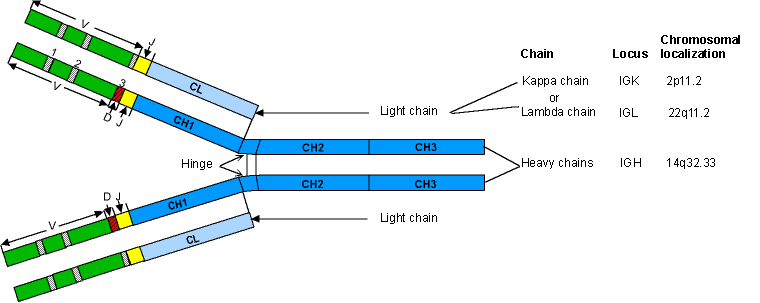
\includegraphics[scale=0.37]{img/angfig1.png}
\end{center}
\caption{Aperçu d'un lymphocyte, et des régions V(D)J sur le site actif.}
\end{figure}

\section{Le projet Vidjil}

\textit{Vidjil} est un projet intra (pour le développement des programmes) et extra (pour toute la partie échantillonage) Universitaire, créé par un petit groupe de chercheurs et d'ingénieurs de l'équipe \textit{Bonsai} et du \textit{Laboratoire d'Hématologie de Lille2}.
\newline
Ce projet a pris naissance en 2011. Peu d'outils fiables et complets étaient disponibles pour le séquençage à haut-débit\footnote{Méthode de séquençage massif de l'ADN, avec clonage et amplification moléculaire - créé en 2005} demandé par l'équipe d'Hématologie de Lille2 pour leurs analyses concernant principalement la L.A.L., menée par \textbf{Claude Preudhomme} - requièrant beaucoup de travail en algorithmique et programmation informatique, ainsi que dans la création et l'adaptation à un modèle biologique spécifique\footnote{Voir le premier article écrit par \textbf{Mathieu Giraud} et \textbf{Mikaël Salson}, sur l'\textit{algorithme}.}.
Après en avoir parlé avec \textbf{Martin Figeac}, cette dernière a de suite émis l'idée d'en discuter avec des informaticiens intéressés par la biologie, issus notamment de l'équipe \textit{Bonsai} du \textit{LIFL} - ce qu'il a fait en parlant du projet à M. \textbf{Giraud} et M. \textbf{Salson}.
Les deux équipes Universitaire se sont donc rencontrées début de l'année 2011 pour en parler. Ce n'est qu'en 2012 que le premier programme a été écrit, et que le projet \textit{Vidjil} a réellement débuté.

Le projet \textit{Vidjil} est principalement conçu pour les médecins et les chercheurs.
\newline 
Il consiste à la mise en place d'un programme permettant de séquencer à haut-débit les clones V(D)J, issus de données d'un format FASTA ou FASTQ\footnote{Les formats FASTA et FASTQ sont des formats de fichier texte utilisés pour stocker des séquences biologiques de nature nucléique ou protéique.}, à partir d'un échantillon de sang d'un patient atteint de L.A.L. (voir \textbf{Figure 2} de la partie \textbf{Annexe}). Le résultat retourné par le programme est donc une analyse de l'échantillon, stockée dans un fichier au format biologique DATA, en utilisant JSON\footnote{JSON est un format de données textuelles et générique, permettant de représenter de l'information structurée. Ce format a été créé par M. \textbf{Douglas Crockford} en 2005.}).Ce programme est écrit en C++, dû à la gestion de la mémoire héritée du langage C, et est dénommé \textit{Vidjil}. Aussi, il consiste en une interface Web (composée majoritairement de Javascript), appelée \textit{interface}, dont le but est d'afficher toutes les informations nécessaires quant aux résultats de séquençage recueillis dans le fichier DATA, et d'en faire une sortie papier au format PDF. L'interface Web a été décidé afin de permettre aux utilisateurs d'avoir le même résultat, et ne pas avoir à installer des packages ou plugins pour l'utiliser à bon escient, sur différents systèmes d'exploitation.
\newline
L'idée sur laquelle repose le projet \textit{Vidjil} est que toutes les informations, quant aux réarrangements V(D)J issus du prélévement de sang, pourront être étudiées, comptées et analysées plus facilement par les utilisateurs du logiciel, afin de pouvoir suivre la maladie, mesurer son étendue, mais aussi adapter les traitements médicaux au mieux et prédire les rechutes.

\begin{figure}[H]
\begin{center}
	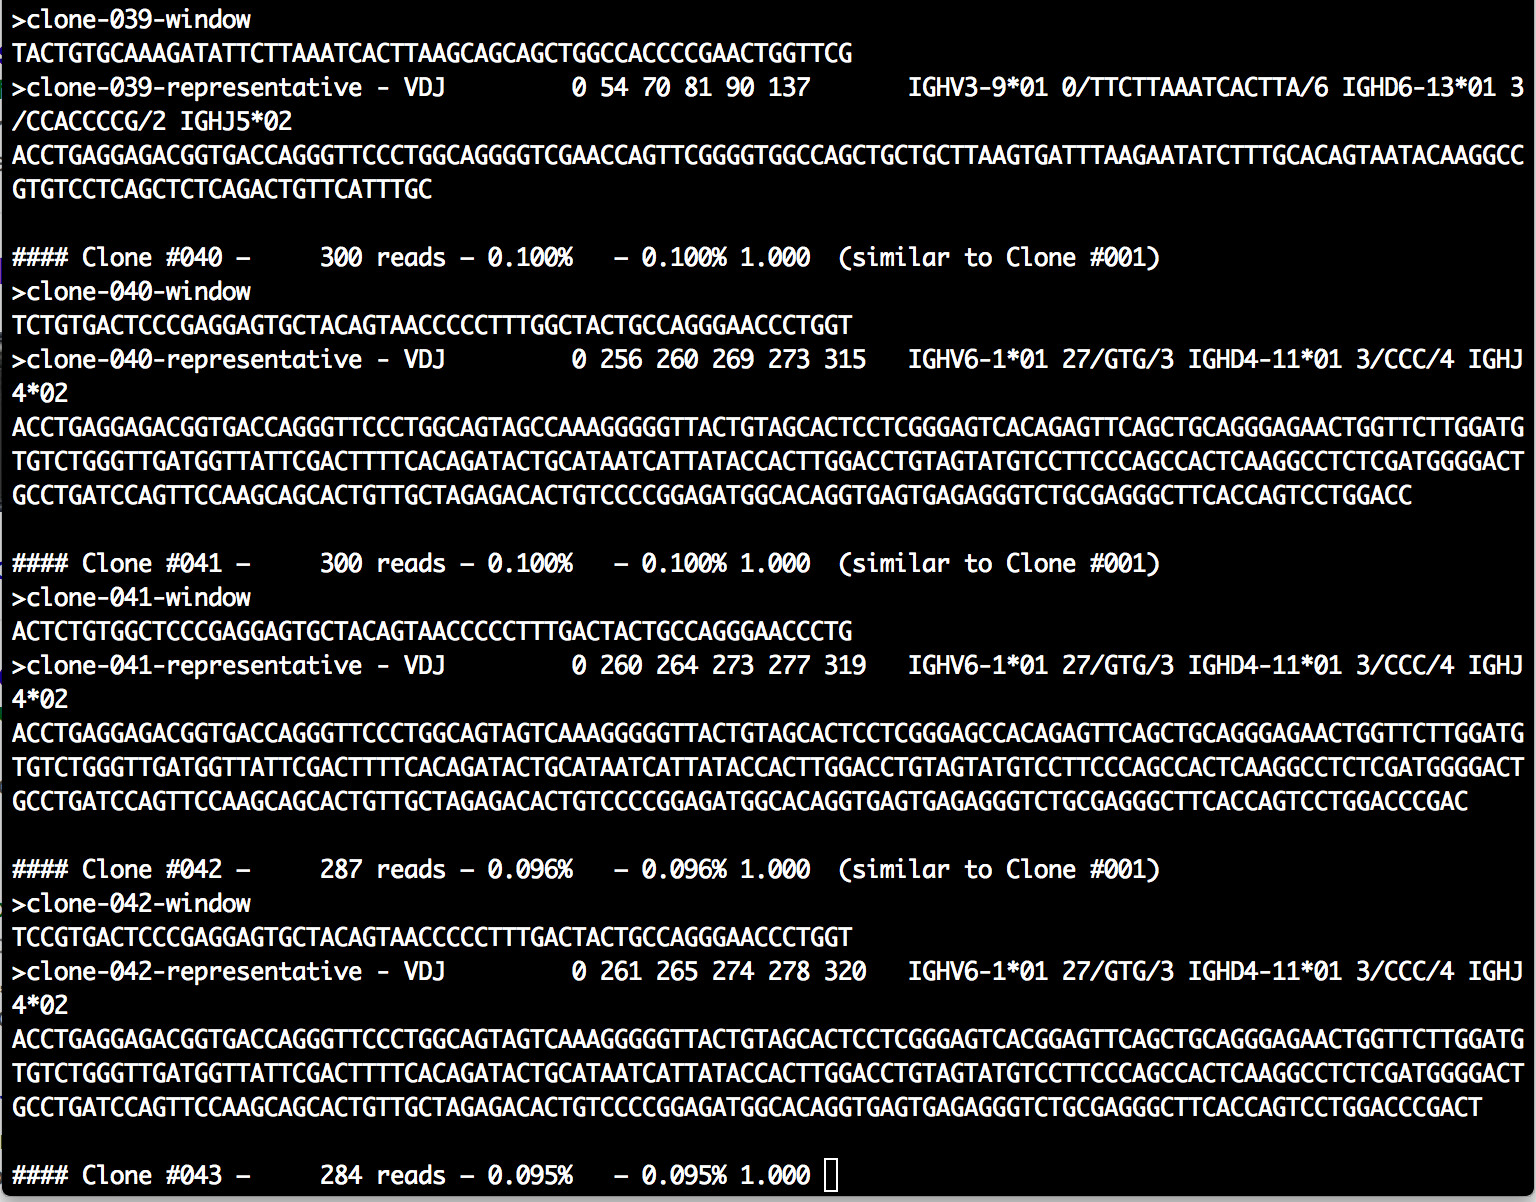
\includegraphics[scale=0.6]{img/C++-Ex.jpg}
\end{center}
\caption{Aperçu d'une segmentation (en cours sur ce \textit{screenshot}), avec \textit{Vidjil}}
\end{figure}

\textit{Vidjil} est donc un projet créé en partenariat avec le \textit{Laboratoire d'Hématologie de Lille2}, par \textbf{Mathieu Giraud}, \textbf{Mikaël Salson} et \textbf{Claude Preudhomme}.
Les deux équipes travaillent aujourd'hui avec \textit{EuroClonality NGS}\footnote{\textit{EuroClonality NGS} est un Consentium Européen contenant plusieurs laboratoires, ce qui est utile au projet quant à l'échantillonage des données.}, ainsi que différents laboratoires Français - comme l'hôpital Necker à Paris ou l'hôpital de Rennes - mais aussi de République Tchèque et d'Angleterre.

\section{Objectifs de stage}
Mes objectifs m'ont été donnés par \textbf{Mathieu Giraud} et \textbf{Mikaël Salson} lors d'un entretien téléphonique et oral en Décembre 2013/Janvier 2014.
\newline
La problèmatique était de permettre à l'utilisateur de l'\textit{interface} de visualiser de façon intéractive les clones V(D)J selon leurs distances d'édition, de façon à suivre la progression des mutations des lymphocytes cancéreux dans le temps.
\newline
Cette problématique devait être résolu \textit{via} deux objectifs, présentés ci-dessous. 

\subsection*{L'\textit{interface}}
Dans un premier temps, je devais intégrer dans l'\textit{interface} un graphe permettant de visualiser physiquement les distances d'édition des clones, ce qui permettrait de percevoir directement la similarité et la disparité des clones.
\newline
Ce premier travail devait s'effectuer sur une durée de deux mois, avec une programmation en HTML5, CSS3 et le langage Less, le langage orienté objet Javascript, Ajax, et en utilisant les frameworks\footnote{Un \textit{framework} est un ensemble d'outils et de composants logiciels organisés conformément à un plan d'architecture et des patterns, l'ensemble formant ou promouvant un "squelette" de programme - il est conçu en vue d'aider les programmeurs dans leur travail.} Javascript D3JS et JQuery - tous ces langages et frameworks étant déjà intégrés à l'\textit{interface}, depuis sa conception par \textbf{Marc Duez}.

\subsection*{DBSCAN}
Deuxièmement, le travail devait déborder sur une partie beaucoup plus algorithmique, avec l'utilisation de DBSCAN\footnote{DBSCAN est un algorithme de partitionnement de données proposé en 1996 par \textbf{Martin Ester}, \textbf{Hans-Peter Kriegel}, \textbf{Jörg Sander} et \textbf{Xiaowei Xu}.} afin de partitionner les clones V(D)J en fonction de deux paramètres: leur distance d'édition, ainsi que leur nombre de voisins.
\newline
L'algorithme était à implanter en Javascript, sur une durée de 1 mois.

\chapter{Préparation}

Avant de me lancer dans le travail tout de suite, il m'a fallu étudier l'\textit{interface}, ses différentes parties afin de savoir le rôle de chacune, mais aussi les langages qui composaient le site internet afin de pouvoir au mieux les exploiter.

\section{L'\textit{interface}}

\subsection{Un travail d'un an...}
Toute la conception et l'écriture du code de l'\textit{interface} ont été effectués par l'ingénieur de recherche du projet \textit{Vidjil}: \textbf{Marc Duez}. 
\newline
M. \textbf{Duez} a commencé à participer au projet \textit{Vidjil} dès Mars/Avril 2013, lors son projet de fin d'année pour le Master MoCAD.
Son ambition était de créer un logiciel répondant aux besoins des médecins et des chercheurs, avec le plus de facilité possible, tout en respectant les principes de "Programmation Orientée Objet"\footnote{Paradigme de programmation informatique.} et de "Modèle-Vue-Contrôleur"\footnote{Modèle destiné à répondre aux besoins des applications interactives en séparant les problématiques liées aux différents composants au sein de leur architecture respective.}.
\newline
À la fin de son Master, il a été embauché dans l'équipe \textit{Bonsai} afin de pouvoir continuer à travailler sur cette même \textit{interface}.

\subsection{Langages et frameworks}
Le programme utilise les langages les plus utilisés du Web: HTML5, CSS3, JavaScript et Ajax.
\newline
Tout le côté "Administration serveur" a été réalisé grâce au langage Python (version 2.7), ainsi qu'au framework \textit{open source} web2py.
\newline
Côté conception, il y avait déjà plus de 20 classes Javascript écrites (à raison de 1000 lignes de code par classe), utilisant 2 \textit{frameworks} JavaScript (re)connus (D3JS et JQuery), ainsi que le langage Less\footnote{Less est un langage dynamique de génération de feuilles de style, conçu par \textbf{M. Sellier Alexis}, très utile quant au changement dynamique de feuille de style afin de mieux visualiser les données calculées pour un échantillonage préparé, et permettant beaucoup plus de souplesse que le langage CSS, permettant de définir la présentation du document HTML.}.

\begin{figure}[H]
\begin{center}
	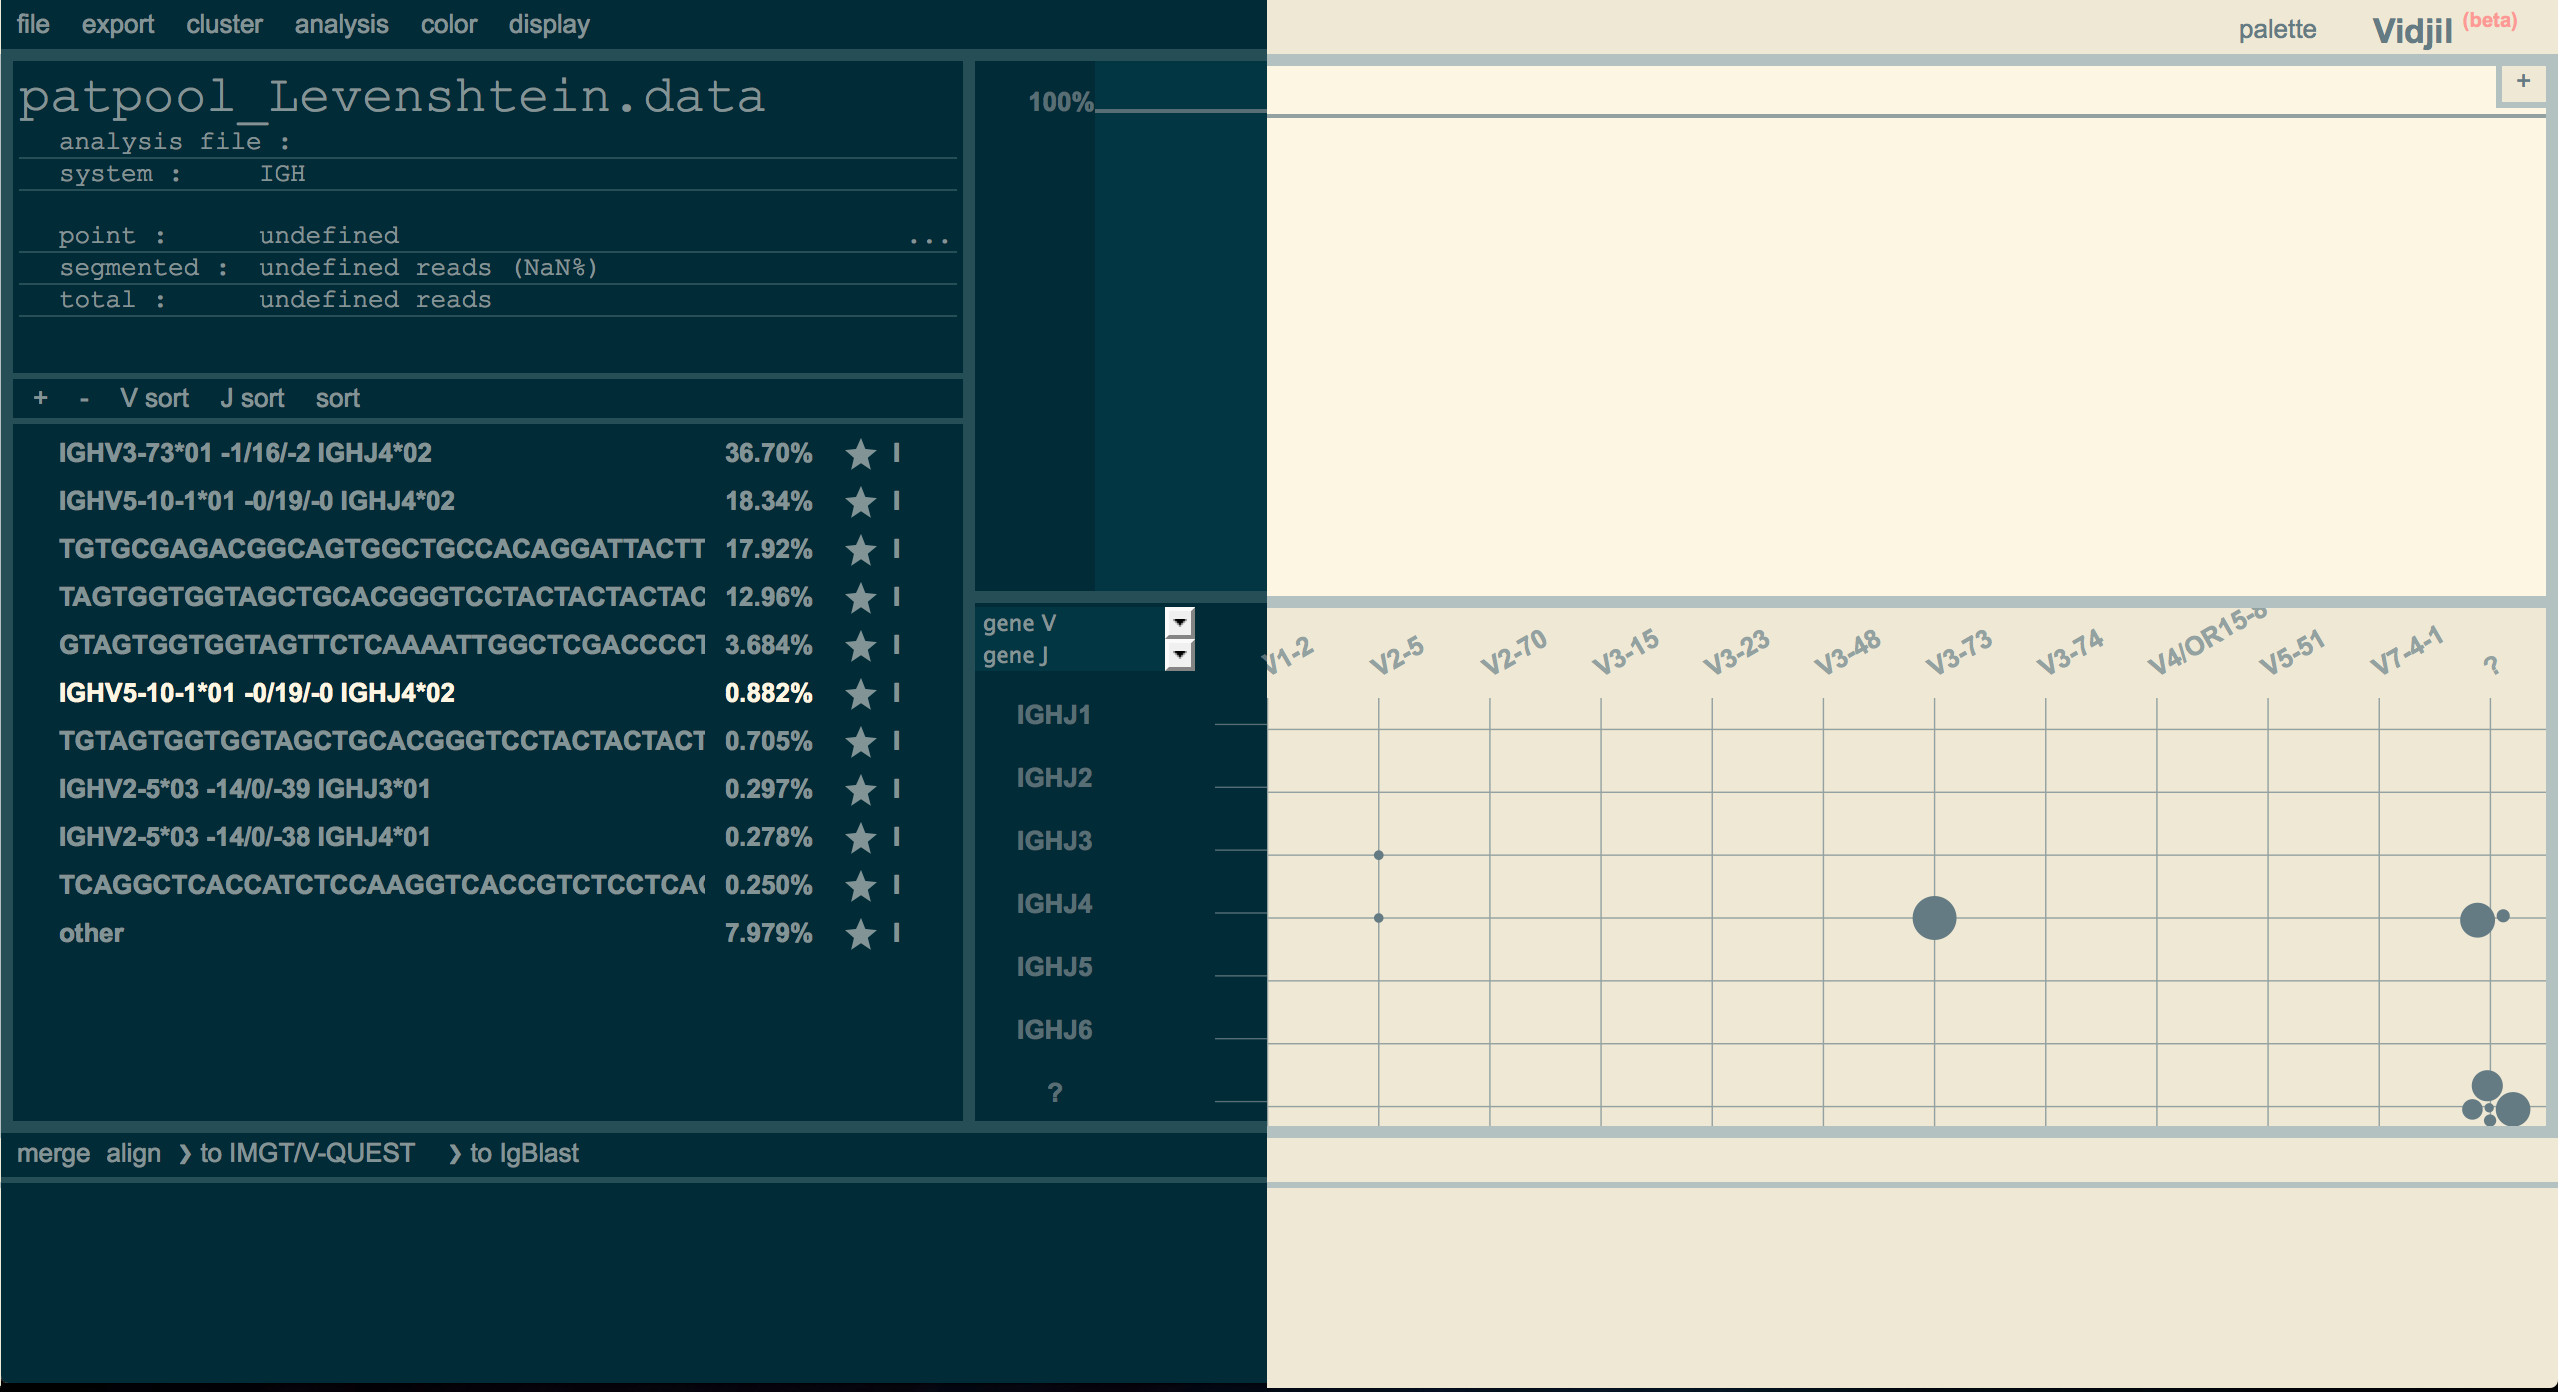
\includegraphics[scale=0.35]{img/Montage_Sans_Annotations.jpg}
\end{center}
\caption{Aperçu général de l'\textit{interface} - montage via \textit{Gimp}, avec les palettes CSS ``Dark'' (à gauche) et ``Light'' (à droite)}
\end{figure}

\subsection{Composition de l'\textit{afficheur}}

L'\textit{interface} se présente sur différentes parties, toutes dépendantes les unes des autres\footnote{Se rapporter à l'annexe, pour une visualisation de l'\textit{afficheur} et ses différentes parties}.
\newline Je ne me suis intéressé, pour mon stage, qu'à trois grandes parties composant celui-ci:
\begin{itemize}
\item{le \textbf{menu haut} - pour l'implémentation des distributions, de la clusterisation et de la colorisation DBSCAN (voir \textbf{Figure 4}),}
\item{l'affichage des informations (\textbf{partie gauche}) - pour l'implémentation de la clusterisation par DBSCAN (voir \textbf{Figure 5}),}
\item{et enfin le \textbf{\textit{scatterplot}} - partie au format \textit{SVG}\footnote{SVG est un format de données conçu pour décrire des ensembles de graphiques vectoriels.} permettant la visualisation des clones selon la distribution, colorisation et/ou clusterisation demandée(s) (voir \textbf{Figure 6}).}
\end{itemize}

\begin{figure}[H]
\begin{center}
	
\includegraphics[scale=0.4]{img/Aff_menu_haut.jpg}
	\caption{\textbf{Menu haut} de l'\textit{interface}}
	\vskip2em
	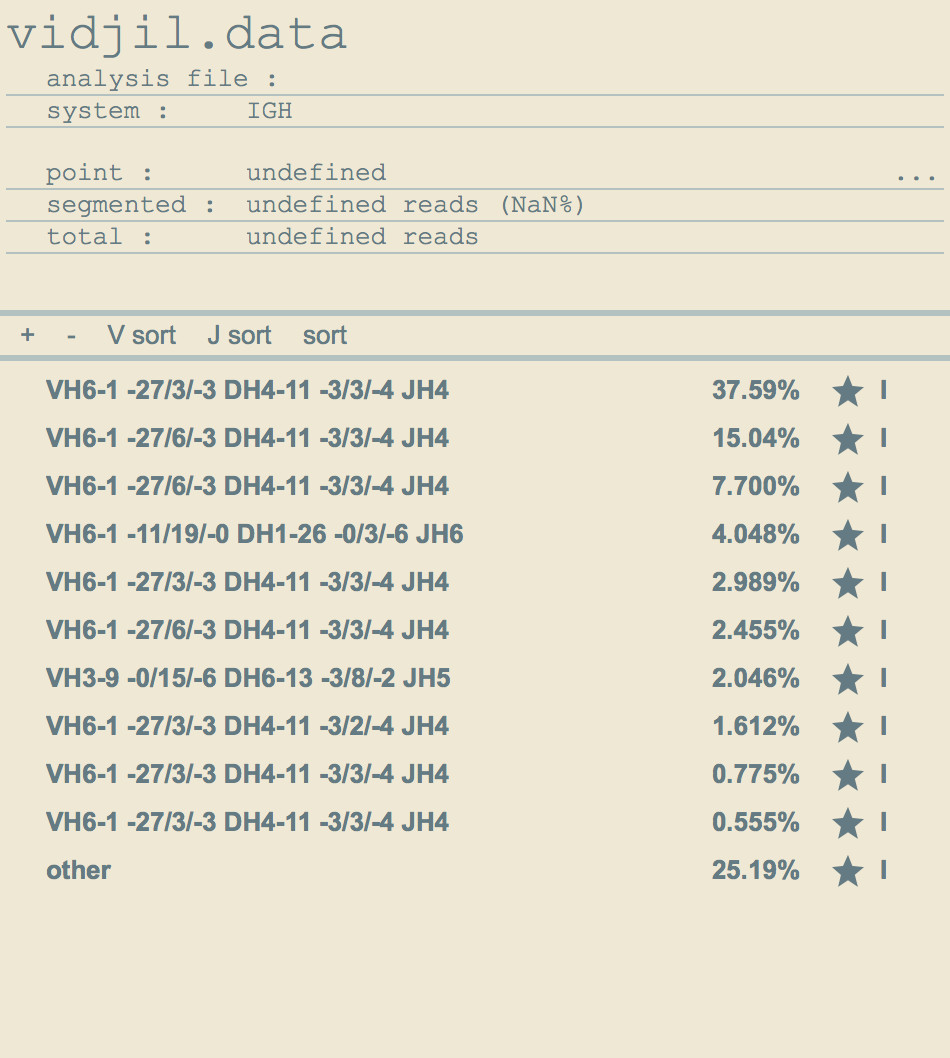
\includegraphics[scale=0.35]{img/Aff_menu_gauche.jpg}
	\caption{Développement des informations (ou \textbf{menu gauche}) de l'\textit{interface}}
	\vskip2em
	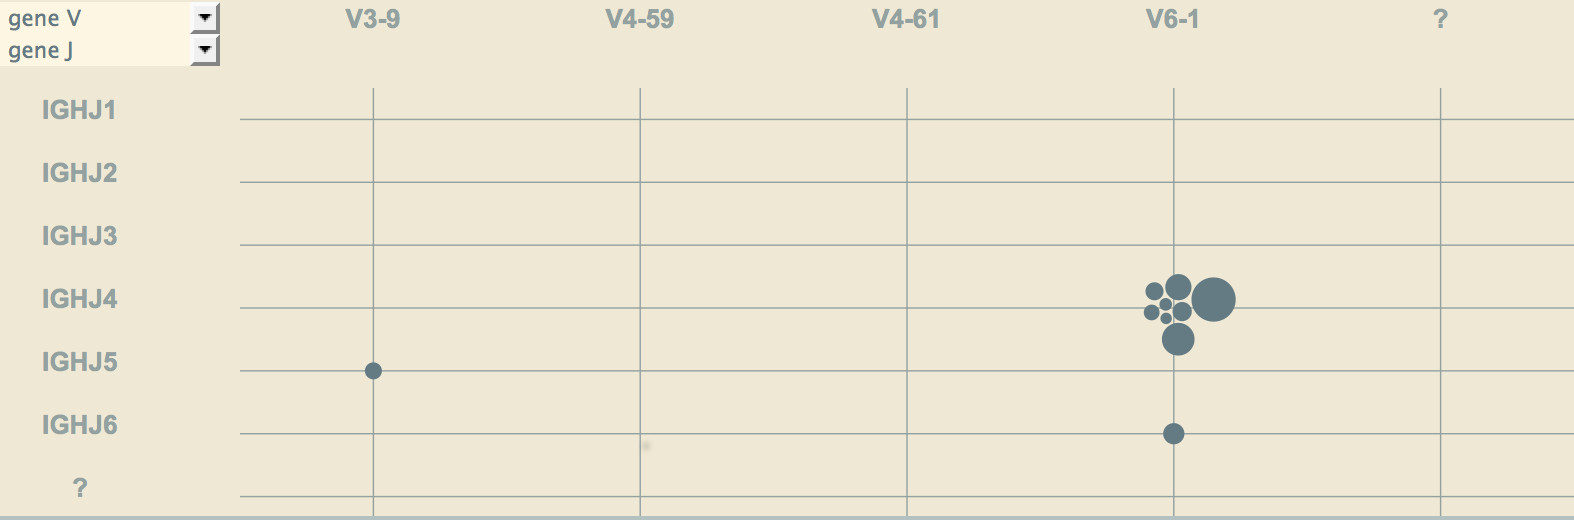
\includegraphics[scale=0.35]{img/Aff_menu_droite.jpg}
	\caption{Le \textbf{\textit{scatterplot}} de l'\textit{interface}}
\end{center}
\end{figure}

\section{Étude et intégration}

Cette phase a duré 2 semaines.

\subsection{La documentation}
Ne connaissant pas les \textit{frameworks} D3JS et JQuery, les langages Ajax ou encore Less, il a donc fallu que je me documente à leur sujet afin de pouvoir exploiter toutes les fonctionnalités implémentées, mais aussi comprendre quand et comment les intégrer au projet.

\subsection{L'intégration au projet}
Durant les deux premières semaines, il m'a fallu étudier tout le code du projet utile à mes objectifs, ainsi que recourir à la création de la documentation pour le développeur (obsolète ou inexistante). L'étude du projet a été pour moi la plus grosse difficulté dans ce stage, n'ayant jamais effectué ceci auparavant, ni obtenu une ou plusieurs méthode(s) pour me permettre d'être le plus efficace possible pour ceci. Aussi, j'ai profité de ce temps afin de corriger plusieurs erreurs mineurs dans l'\textit{interface}, afin de me permettre de mieux discerner les grandes parties de celle-ci et leurs buts respectifs.
\newline
De plus, il était très important pour moi de respecter les règles de l'équipe en matière d'ingénierie logicielle, ne serait-ce par l'écriture du code, de la documentation, mais aussi par rapport au respect des \textit{commits}\footnote{Un \textit{commit} est une action permettant d'envoyer ses modifications locales vers le référentiel central}/\textit{push}\footnote{Un \textit{push} est une action permettant de transférer des commits d'un dépôt local à un dépôt distant} sur le serveur, via le logiciel de gestion de versions décentralisé \textit{Git}\footnote{\textit{Git} est un logiciel libre créé par \textbf{Linus Torvalds}, permettant de gérer très facilement les codes sources de projets.}.

\subsection{Le domaine biologique}
Enfin, je me suis remis à étudier par moi-même la microbiologie, le principe de recombinaison V(D)J, ainsi que les techniques de séquençage et de clusterisation. Tout celà afin de me permettre de comprendre et de poursuivre les discussions lors des réunions dans l'équipe, et avec le \textit{Laboratoire d'Hématologie de Lille2}.

\chapter{Le graphe de distances d'édition}

Le projet contenait, à mon arrivée, 5 distributions\footnote{Une distribution est une visualisation possible des données, pour une utilisation spécifique.}:
\\[2mm]
\begin{minipage}{0.5\textwidth}
\begin{itemize}
\item V/J génique,
\item V/J allèlique,
\item longueur des régions V/N,
\item abondance des régions V et J,
\item histogramme d'abondance des régions V.
\end{itemize}
\end{minipage}
\begin{minipage}{0.5\textwidth}
	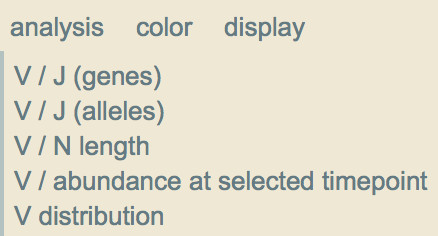
\includegraphics[width=\textwidth]{img/5distributions.jpg}
	\\
\end{minipage}


Toutes ces distributions sont nécessaires à l'utilisateur, afin de visualiser directement la disparité et le réarrangement des clônes, en fonction d'un jeu de données au format biologique DATA. Or, il n'y avait pas encore de travaux effectués sur une distribution des clones en fonction de leurs distances d'édition, afin de pouvoir visualiser leur rapprochement en fonction de leurs disparités et ressemblances nucléotidiques, essentielle pour un suivi des lymphocytes cancéreux dans le temps.

\section{Ajout d'une nouvelle distribution}
L'ajout d'une nouvelle distribution n'était pas aisée, pour différentes raisons techniques.

Il a d'abord fallu me plonger dans le code du \textit{scatterplot} afin de prévisualiser où implanter ma distribution, et quelles modifications seraient à effectuer sur cette partie de l'\textit{interface}. Le moteur de D3JS, initialement, ne pouvait que positionner les clones à une place donnée, et se charger de tous mouvements associés à ceux-ci. Pour cette distribution, il fallait forcer le moteur physique de D3JS afin qu'il puisse positionner les clones \textbf{lui-même, le plus précisémment possible} (c'est à dire en respectant au maximum toutes les distances définies entre chaque clone), ne pouvant prédestiner la position des clones et de ses voisins sans distances - celà n'aurai alors aucune utilité d'implanter cette distribution.

\section{Création du graphe}

D3JS contient absolument toutes les fonctions nécessaires afin de construire proprement un graphe - un soucis concernera cependant le respect exact des informations données, et de la transformation effectuée par son moteur physique, ce qui a été précedemment évoqué.
\newline
Voici les transformations effectuées sur le moteur physique:
\begin{itemize}
\item{ajout d'une durée d'animation élevée,}
\item{ajout d'une gravité,}
\item{ajout d'arêtes via un tableau Javascript (dans le fichier au format DATA) ayant comme entrées:	
\begin{itemize}
\item{un point source,}
\item{un point cible,}
\item{une longueur entre ces deux points}
\end{itemize}
, et de distances spécifiques pour chacune,}
\item{d'une élasticité - ce paramètre sera détaillé dans la sous-partie consacrée aux \textbf{Résultats}}
\item{ajout d'une liaison entre un point et un début d'arête, afin de pouvoir bouger les arêtes en même temps que le point.}
\end{itemize}

\section{Problème et résolution des arêtes}

Sur un graphe à 100 clones, chacun était lié aux 99 autres par une arête, il faudra donc créer un graphe complet à 10000 arêtes. 
Je me suis alors posé la question suivante: "Le moteur physique sera-t-il capable de prendre en compte un nombre aussi élevé d'arêtes, ainsi que le calcul nécessaire pour la mouvance du graphe complet, en temps réel?"
Après plusieurs tests, la réponse est \textbf{non}: il n'a pas été créé et optimisé pour une tâche aussi lourde.

Il a donc fallu trouver un moyen d'optimiser au maximum la composition du graphe (c'est à dire garder un nombre minimal d'arêtes), afin de le représenter le plus rapidement possible, avec un maximum de concordance et de respect par rapport aux données fournies.
Les 3 solutions présentées ci-dessous implémentent cette idée de réduire drastiquement le nombre d'arêtes, sans diminuer la qualité du graphe.

\subsection{\textit{"Il était une fois, un premier algorithme..."}}
Le premier algorithme qui m'est venu à l'esprit est de supprimer toutes les arêtes ayant une longueur supérieure à une distance implantée en dur dans le programme - cela permettra donc d'alléger le tableau d'arêtes Javascript pris en compte par le moteur, et de moins le faire souffrir lors des calculs.

Ce procédé a été un semi-échec: sur plusieurs jeux de données, nous avons supprimé en moyenne un peu plus de 50\% des arêtes disponibles (nous étions passé de 10000 à 4970 arêtes sur un jeu de données, pour citer un exemple) - malheureusement, le moteur peinait à calculer toutes les positions des noeuds et arêtes par \textit{frame} une nouvelle fois (sur une machine à processeur corei5 à 8Go de RAM, GPU Intel HD 4000 intégré).
Il était donc nécessaire de chercher un nouvel algorithme qui pourrait, au moins, diviser de moitié le nombre d'arêtes qui seront à prendre en compte par le moteur. Cependant, l'idée de modifier la distance maximale d'arêtes à afficher a été validé et gardé dans le projet - elle a été implémenté sous la forme d'un \textit{slider}, présent dans le sous-menu "Display" du \textbf{menu haut}.

\begin{figure}[H]
\begin{center}
	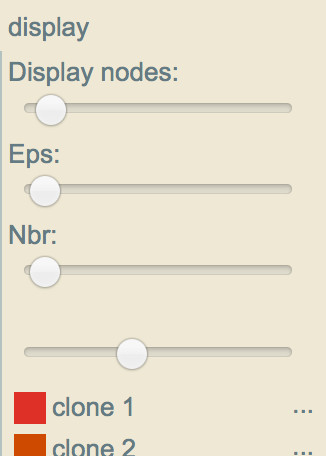
\includegraphics{img/Aff_menu_display.jpg}
\end{center}
\caption{Sous-menu "Display" du menu haut avec, de haut en bas: le \textit{slider} "Display nodes" permettant d'afficher ou non un nombre plus ou moins grand de clones, les deux \textit{sliders} permettant de changer les paramètres de DBSCAN, et enfin le \textit{slider} pour modifier la distance maximale d'affichage des arêtes (pour le graphe concernant les distances d'édition)}
\end{figure}

\subsection{\textit{"L'algorithme contre-attaque"}}
Le deuxième algorithme a été proposé par M. \textbf{Duez Marc}; beaucoup plus brutal, il permet de dispenser une grande partie d'arêtes, considérées comme inutiles lors de la construction du graphe - toujours en fonction des distances.
\newline
Il s'agit de:
\begin{enumerate}
\item trouver les 3 plus grandes arêtes du graphe ayant les caractéristiques suivantes:
	\begin{itemize}
	\item chaque arête ne doit pas avoir de point commun avec les autres,
	\item chaque point à une distance minimale d'une extrêmité d'une arête trouvée ne doit plus être prise en compte lors du calcul,
	\item chaque arête doit être le moins parallèle possible des autres,
	\end{itemize}
\item calculer toutes les arêtes possibles entre une extrémité d'arête trouvée,
\item calculer 4 ou 5 arêtes possibles, dans une distance minimale, des points trouvés lors de l'étape 2.
\end{enumerate}
Le résultat a été concluant - en effet, en déroulant l'algorithme, nous pouvons voir que:
\begin{itemize}
\item l'étape 1 se fera avec un maximum de 3 arêtes,
\item l'étape 2 se fera avec un maximum de 600 arêtes (au total: 600 + 3 arêtes),
\item l'étape 3 se fera avec un maximum de 100 * 5 arêtes (au total: 1103 arêtes maximum).
\end{itemize}
Ainsi, nous avons pu enlever un peu moins de 90\% des arêtes totales pour un jeu de données quelconque, en moyenne; ce qui nous est très bénéfique par rapport au temps de calcul du moteur pour chaque \textit{frame}. Malheureusement, malgré un bénéfice de mémoire et calcul, le respect de la structure du graphe n'était pas optimal.

\subsection{\textit{"Le carré est un triangle qui a réussi, ou une circonférence qui a mal tourné..."}}\footnote{Citation de \textbf{Pierre Dac}}
Le troisième algorithme a été proposé par M. \textbf{Giraud Mathieu}. C'est cet algorithme qui a été retenu par mon équipe et moi-même, car respectant aussi bien la structure, que consommant moins de mémoire et de temps de calcul.
\newline
Cet algorithme modifie seulement la 1ère partie de l'algorithme précédent, de sorte à ne prendre que les 3 plus grandes arêtes formant un triangle, dont la somme des côtés sera la longueur maximale de toutes les autres représentations triangulaires possibles, selon les données initialement recueuillies. Ainsi, chaque noeud du triangle est une source d'une arête, mais aussi une cible d'une autre, ce qui nous assurerera d'avoir une structure triangulaire: un "squelette" du graphe, pour l'aider le moteur à mieux modéliser la "chair".

\section{Résultats}

Le résultat final montre bien les similarités entre les différents clônes calculés, très rapidement. Cependant, les résultats ne sont pas à la hauteur de nos espérances, encore à cause d'un soucis de représentation.
En effet, celle-ci ne préserve pas de façon optimale les distances données en entrée. Étant donné qu'il place par lui-même chaque clone, il le fera au fur-et-à-mesure de la lecture (par un ordre quelconque) des distances d'édition du tableau Javascript, et les prendra en compte de moins en moins.

\begin{figure}[H]
\begin{center}
	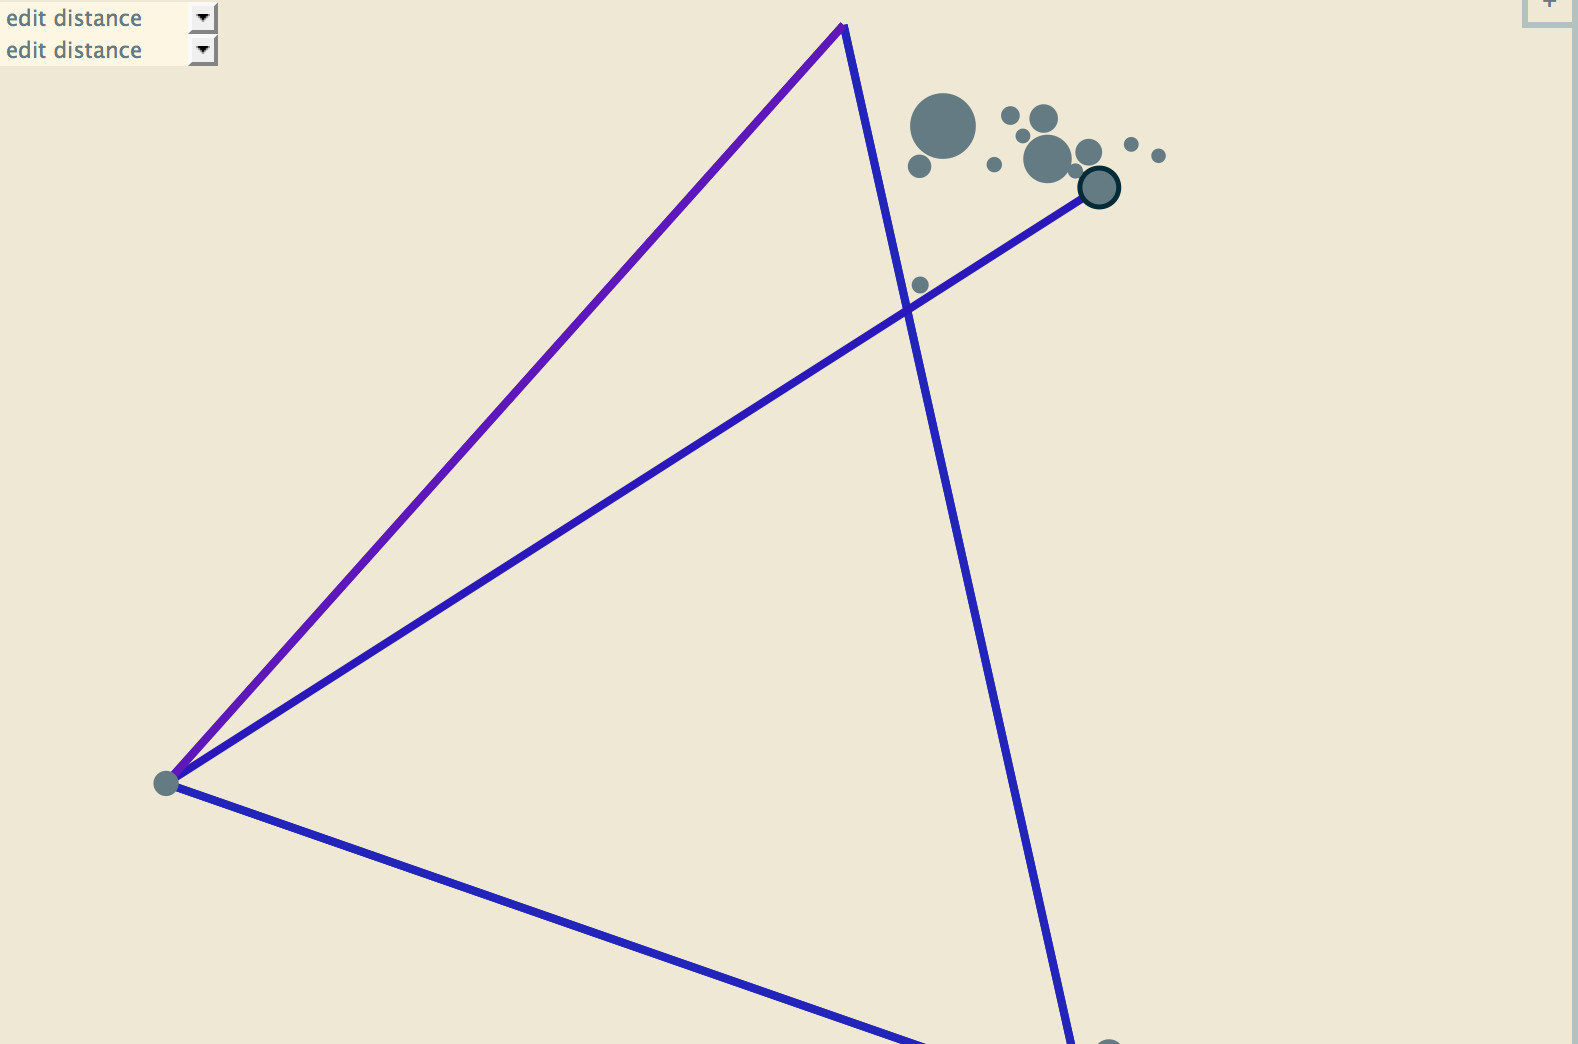
\includegraphics[scale=0.5]{img/Edit-Distance-Ex.jpg}
\end{center}
\caption{\textit{Afficheur} avec la distribution de distances d'édition}
\end{figure}

Nous nous intéressons plus particulièrement à la similarité des clones qu'à leur disparité. Il était donc extrêmement important de garder les arêtes les plus petites (signe que la similarité est élevée) - ainsi, les plus petites arêtes doivent être plus respectées que les plus grandes, sauf pour les arêtes constituant le triangle initial bien entendu. La dernière solution à apporter était de donner une élasticité aux arêtes. Après les tests, il se trouve que les similarités sont bien respectées dans le graphe, mais accompagne un nouveau problème. Celui-ci, découlant de la précédente solution, est que les plus grandes distances ne sont plus respectées. Ainsi, deux points ayant une distance d'édition très grande peuvent se retrouver à proximité dans le graphe vu que le moteur attribue par lui-même les positions des clones, dans le \textit{scatterplot}. Ce problème étant, à cause de ce problème par le moteur physique, insoluble, le déploiement du graphe de distances d'édition est un semi-échec.

Il existe cependant 2 solutions à apporter, pour un prochain sujet:
\begin{itemize}
\item{aborder le soucis comme non pas un seul graphe, mais un ensemble de sous-graphes dont le seul paramètre de variation sera la distance d'édition à prendre en compte - variable grâce au \textit{slider} déjà implanté dans l'\textit{interface} pour cette utilisation,}
\item{ne pas développer cet objectif comme un graphe mais plutôt comme un arbre, permettant toujours de répondre à la principale problèmatique - comme un arbre phylogénétique. Ce modèle pourra être implanté avec le \textit{framework} D3JS.}
\end{itemize}

\begin{figure}[H]
\begin{center}
	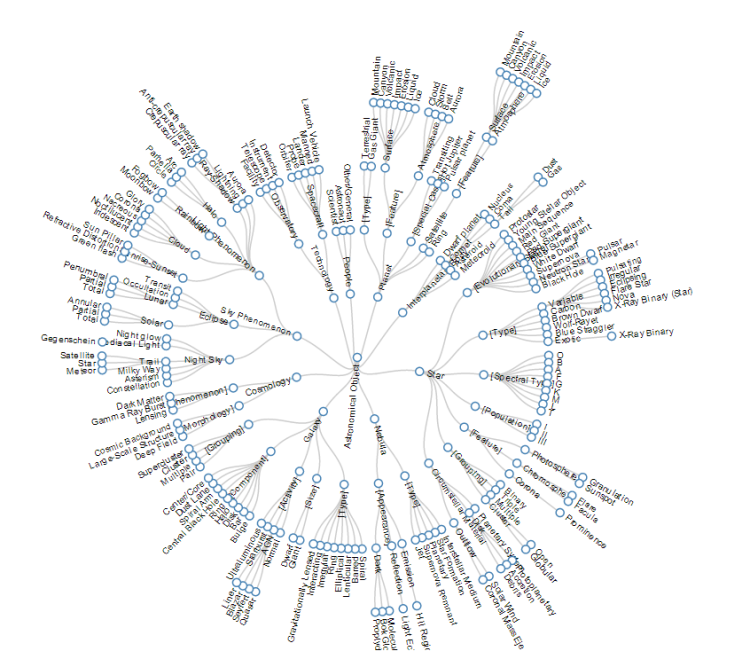
\includegraphics[scale=0.6]{img/phylogenetic_tree_d3js.png}
\end{center}
\caption{Exemple d'implantation d'un arbre phylogénétique circulaire, avec D3JS.}
\end{figure}

\chapter{L'algorithme de clusterisation DBSCAN}

Ce chapitre conduira mon travail et mes réflexions sur la deuxième partie du stage que je devais effectué: l'intégration de l'algorithme de clusterisation DBSCAN (\textit{Density-Based Spatial Clustering of Applications with Noise}).

Ce travail a été réalisé en deux semaines, de fin Mai à la deuxième semaine de Juin.

\section{Présentation}

DBSCAN est un algorithme permettant la clusterisation de données, proposé en 1996 par Messieurs \textbf{Ester Martin}, \textbf{Kriegel Hans-Peter}, \textbf{Sander Jörg} et \textbf{Xu Xiaowei}, s'appuyant sur la densité estimée des clusters à partitionner.
Cet algorithme est très simple à implémenter.
\newline
Tout d'abord, il faut choisir deux paramètres, essentiels à la clusterisation:
\begin{itemize}
\item{\textbf{une distance} ($\epsilon$), représentant un rayon de cercle et qui nous aidera à considérer qu'un point situé à une distance (la distance d'édition ici) inférieure ou égale à $\epsilon$ d'un autre point est représentatif d'un seul cluster},
\item{\textbf{un nombre minimum de points} (\textit{Mp}), que l'on utilisera pour considérer le point pris en compte comme un \textbf{point central} (\textit{\textbf{core point}} - le point détient un nombre de voisins plus élevé que \textit{Mp}, dans le rayon $\epsilon$), un \textbf{point de bordure} (\textit{\textbf{border point}} - le point détient un nombre de voisins moindre que \textit{Mp}, mais est voisin d'un \textbf{point central}), ou encore un \textbf{point de bruit} (\textit{\textbf{noise point}} - tout point n'étant pas l'un des deux précédemment évoqué).}
\end{itemize}

\begin{figure}[H]
\begin{center}
	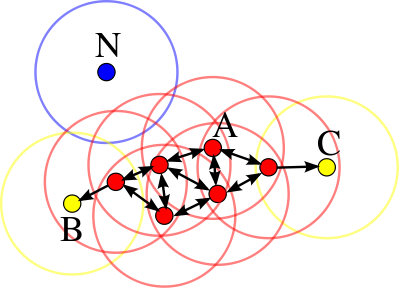
\includegraphics[scale=0.45]{img/400px-DBSCAN-Illustration.png}
\end{center}
\caption{Exemple de clusterisation, avec DBSCAN}
\end{figure}

Cet algorithme est intéressant car il nous permet de parcourir chacun des points d'un graphe, son voisinage, et de clusteriser chaque point en fonction des deux paramètres énoncés précédemment - la densité revient donc au nombre de points (\textit{Mp}) compris dans un rayon bien spécifié ($\epsilon$).

\textbf{\underline{Remarque}}: Il est intéressant de constater que DBSCAN partitionne les données selon une certaine densité, donnée en paramètre via $\epsilon$ et \textit{Mp}; cet algorithme ne pourra donc pas gérer les clusters de densités différentes en même temps (ce qui ne nous intéresse pas ici, fort-heureusement).

L'énome apport de l'implémentation de DBSCAN est de \textbf{regrouper les clones similaires par rapport aux distances d'édition, et son voisinage}, ce qui n'était pas possible avec les précédentes distributions.
Ainsi, cette implémentation de l'algorithme dans l'\textit{interface} permettra à l'utilisateur de pouvoir visualiser directement quels sont les clones les plus similaire, par le rassemblement de ceux-ci, et ainsi de pouvoir déceler les clones cancéreux ayant subi une mutation au cours du temps, et ainsi de marquer l'évolution de la maladie (les distances d'édition étant calculées par rapport aux \textit{windows}, marqueur d'évolution temporel - voir le \textbf{chapitre 5}).
\newline
L'algorithme est représenté ci-dessous (issu de Wikipedia\footnote{\url{http://fr.wikipedia.org/wiki/DBSCAN}}).

\begin{pseudocode}{DBSCAN}{D, eps, MinPts}
\COMMENT{Base de l'algorithme}\\
C $=$ 0\\
$Pour chaque point $P$ non visité des données $D\\
$marquer $P$ comme visité$\\
PtsVoisins$ = $\CALL{epsilonVoisinage}{P, eps}\\
\IF tailleDe(PtsVoisins) < MinPts
\THEN $marquer $P$ comme "bruit"$
\ELSE 
	\BEGIN
		C$++$\\
		\CALL{extensionCluster}{D, P, PtsVoisins, C, eps, MinPts}\\
	\END\\
\\

\COMMENT{Procédure permettant d'inclure un point dans un cluster - extension d'un cluster}\\
\PROCEDURE {extensionCluster}{D, P, PtsVoisins, C, eps, MinPts}
	$Ajouter $P$ au cluster C$\\
	\FOREACH P' \in PtsVoisins \DO
			\IF P'$ n'a pas été visité$
			\THEN 
				\BEGIN
					$Marquer $P'$ comme visité$\\
					PtsVoisins'$ = $ \CALL{epsilonVoisinage}{D, P', eps}\\
					\IF tailleDe(PtsVoisins') >= MinPts
					\THEN PtsVoisins$ = $PtsVoisins \cup PtsVoisins'\\
				\END\\
			\IF P'$ n'est membre d'aucun cluster$
			\THEN $Ajouter $P'$ au cluster $C
\ENDPROCEDURE

\COMMENT{Procedure retournant tous les points de $D$ qui sont à une distance inférieure à $eps$ de $P$}\\
\PROCEDURE{epsilonVoisinage}{D, P, eps}
	$Retourner tous les points de $D$ qui sont à une distance inférieure à $eps$ de $P
\ENDPROCEDURE
\end{pseudocode}

\section{Implantation de DBSCAN}

DBSCAN étant réutilisable à souhait dans le projet, son implémentation aura sa propre classe dans l'\textit{interface}, communiquant avec le Modèle du \textit{"MVC"}\footnote{"Modèle-Vue-Controleur"}.
À l'aide de QUnit\footnote{QUnit est un \textit{framework} permettant d'implémenter des tests unitaires, développé par l'équipe ayant créé le \textit{framework} JQuery.}, j'ai pu créer une série de tests unitaires\footnote{Un test unitaire est une procédure permettant de vérifier le bon fonctionnement d'une partie précise d'un logiciel ou d'une portion d'un programme.} (voir \textbf{Figure 13} dans la partie \textbf{Annexe}) permettant de démontrer la fonctionnalité totale de l'algorithme, sur un jeu de tests (écrit à la main) permettant de tester tous les cas possibles issus d'un jeu de données biologiques.

\subsection{Choix des paramètres}

Les paramètres pris par défaut sont de 0 pour $\epsilon$ et \textit{Mp}. Ainsi, au départ, étant donné que la distance d'édition maximale pour clusteriser est nulle, chaque clone a son propre cluster.
\newline
Le meilleur moyen pour l'utilisateur de réaliser, pour un jeu de données, la meilleure clusterisation est de faire varier les paramètres par nos propres moyens.
J'ai donc ajouté, pour cet usage, deux sliders dans l'\textit{interface} (voir \textbf{Figure 7}).
Ces sliders créent, à chaque modification apportée, un nouvel objet DBSCAN selon les paramètres voulus - ce qui permet de visualiser, en une fraction de seconde, les modifications apportées manuellement.

\begin{figure}[H]
\begin{center}
	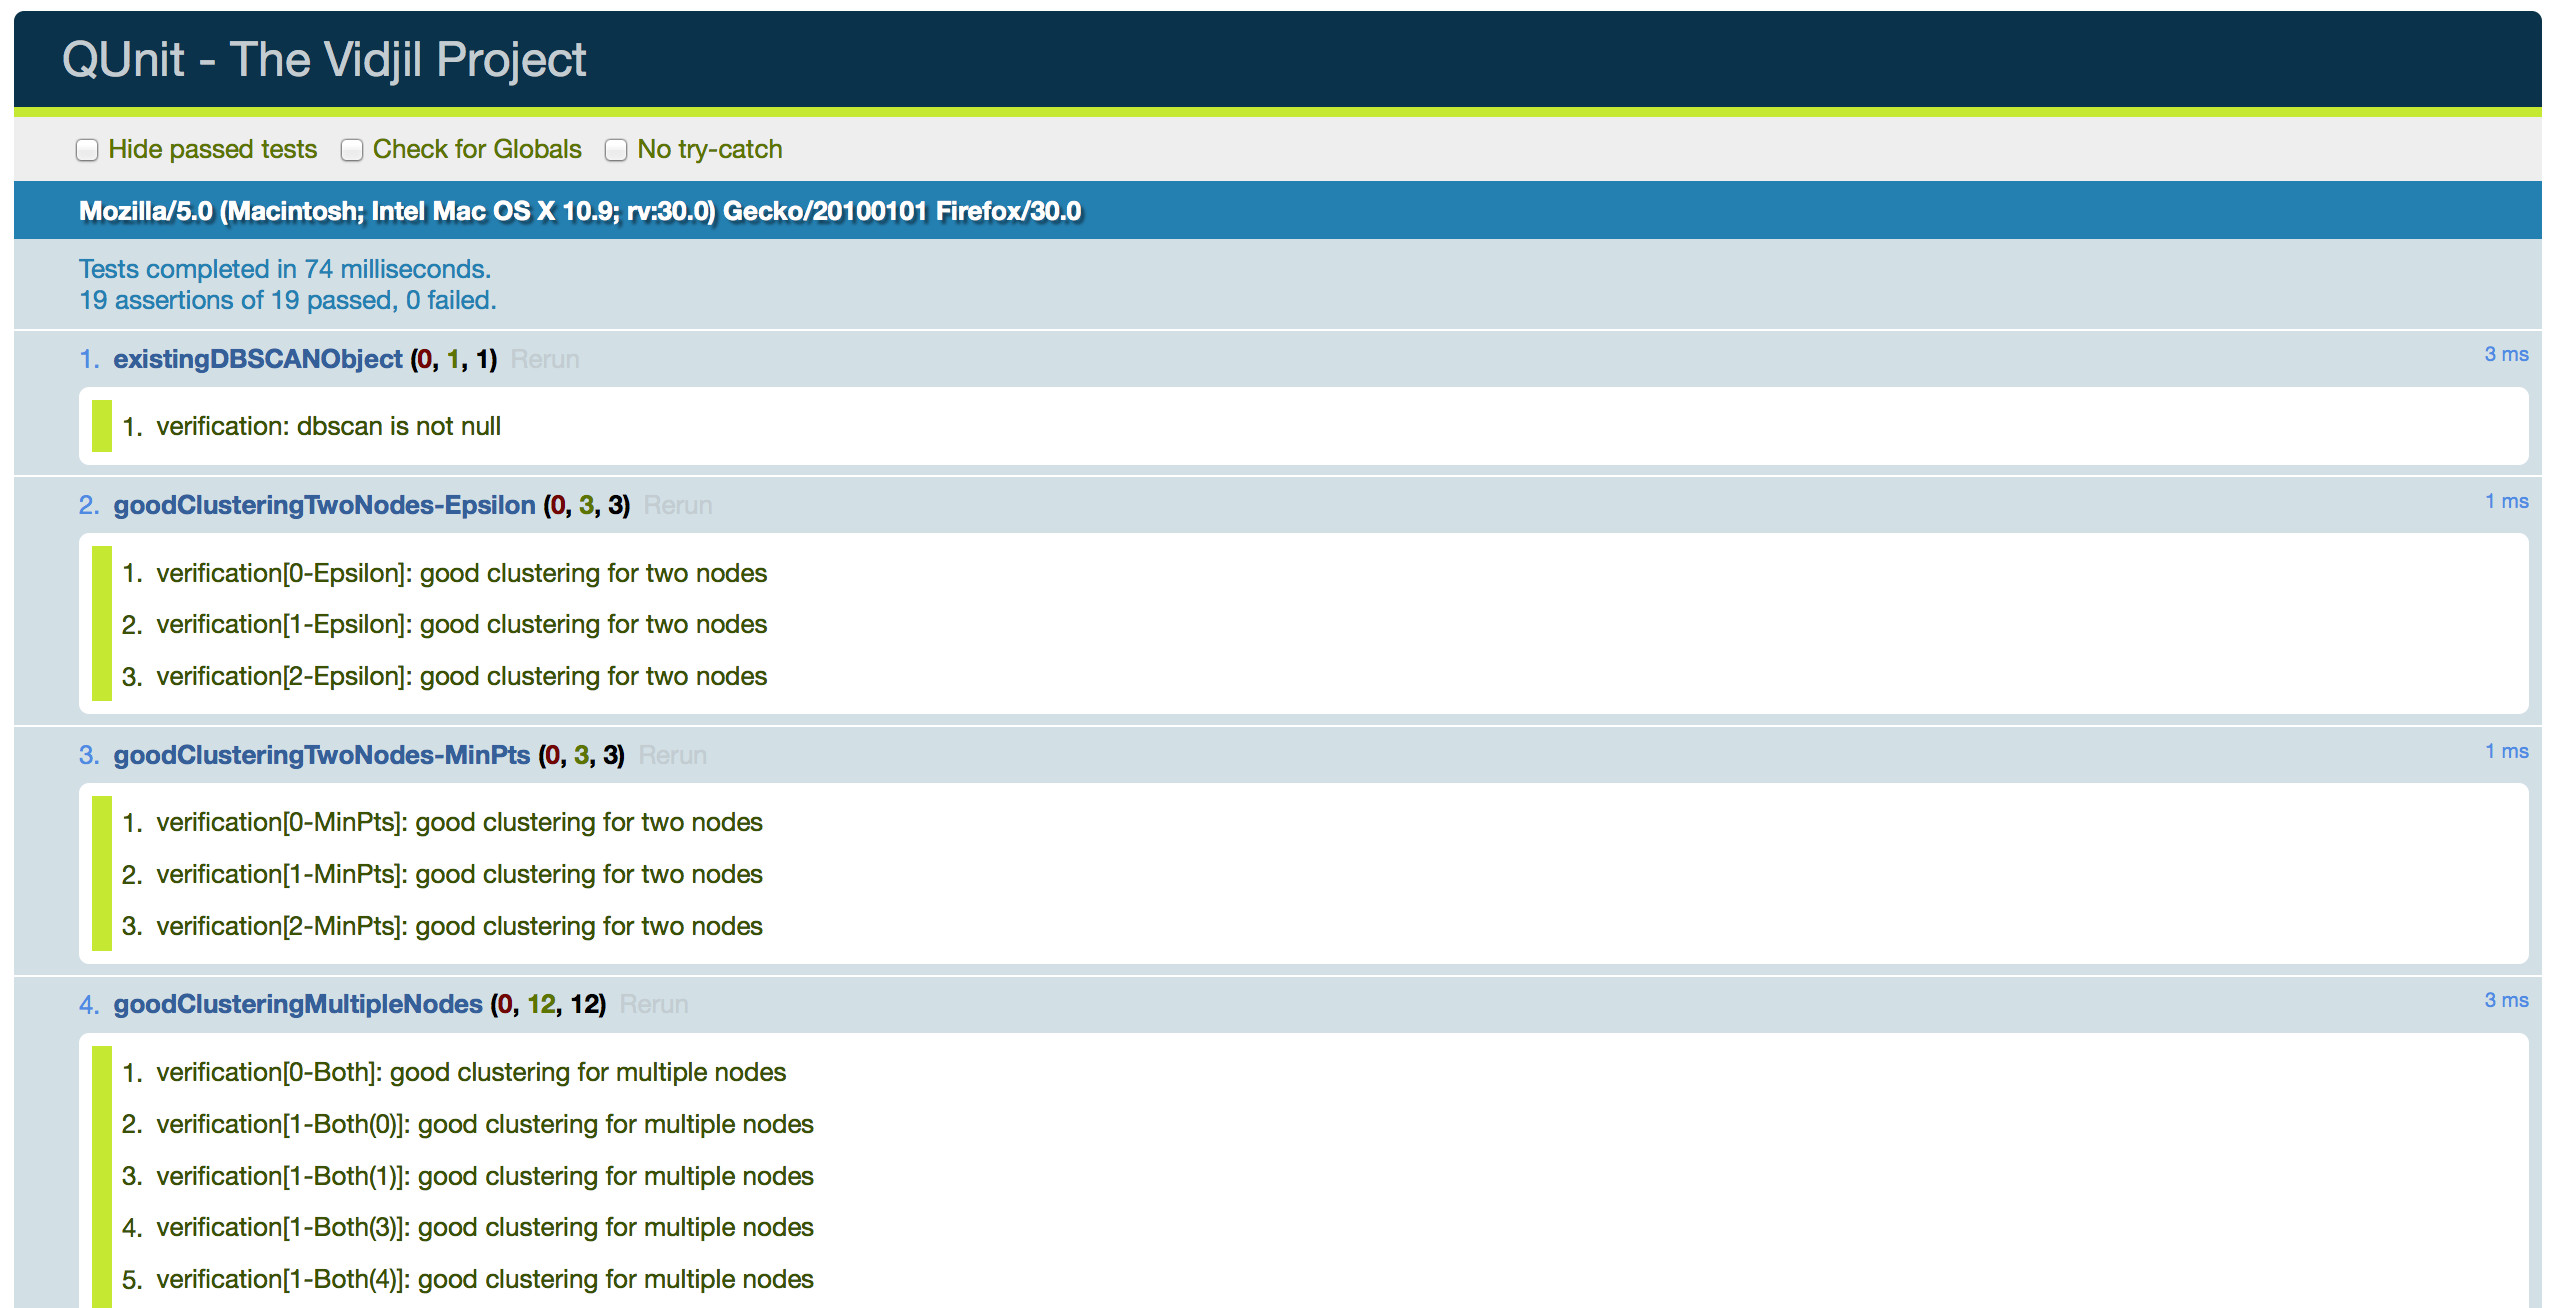
\includegraphics[scale=0.35]{img/QUnit.jpg}
\end{center}
\caption{Interface de QUnit, les tests étant passés avec succès}
\end{figure}

\subsection{Visualisation}

La visualisation des groupes de clones est primordiale - elle en est même la base du sujet de stage. J'ai donc travaillé, une fois l'implémentation terminée de l'algorithme, sur la visualisation du résultat retourné par l'algorithme. Les clusters sont à eux-seuls de tous petits graphes complets dans le cadre \textit{SVG}, ce qui le différencie bien du premier sujet, qui était à lui-seul un seul et même graphe. Ici, nous ne tenons pas compte de la restitution des distances d'édition sur les clusters, étant donné que nous souhaitons juste rassembler les clones et non pas les comparer! J'ai ainsi établi un nouveau paramètrage du moteur pour cette distribution, ne gérant pas la gravité, la restitution des exactes distances d'édition, ainsi que l'élasticité.
\newline
Je me suis alors demandé quelle était la meilleure visualisation possible afin de percevoir les différents clusters - sans aucun doute, la couleur. Chaque clone appartenant à un cluster calculé lors du calcul par l'algorithme, chaque cluster pourra donc avoir une couleur bien spécifique qui pourra donc la distinguer des autres clusters.

La colorisation est beaucoup plus bénéfique visuellement et résiduelle dans le temps (il est en effet possible de colorer les clones selon les résultats de DBSCAN, tout en étudiant une distribution quelconque).
\newline
Aussi, il a fallu faire attention à plusieurs choses:
	\begin{itemize}
		\item{la couleur choisie pour chaque cluster est comprise entre 0 et 270 selon \textit{RGB}\footnote{\textit{RGB}: \textit{Red}, \textit{Green}, \textit{Blue}} - afin d'aller d'une teinte rouge (0) vers le violet (270), des couleurs déjà utilisées dans le projet, et permettant aussi de respecter scrupuleusement la légende des couleurs déjà établie par l'ingénieur de recherche du projet,}
		\item{il a fallu faire attention à ce que les noeuds se ressemblant n'aient pas une teinte beaucoup trop proche l'une de l'autre, afin de permettre une visualisation non-faussée.
			\newline
			Pour palier à ce problème, j'ai donc créé un objet tableau à N entrées (100 ici, pour utiliser au maximum 100 clusters, soit 1 clone par cluster) représentants chaque cluster et une couleur, que j'ai mélangé via l'\textbf{algorithme de Fisher-Yates} (encore appelé \textbf{mélange de Knuth}), très utilisé dans ce genre de situation.}
	\end{itemize}

\begin{figure}[H]
\begin{center}
	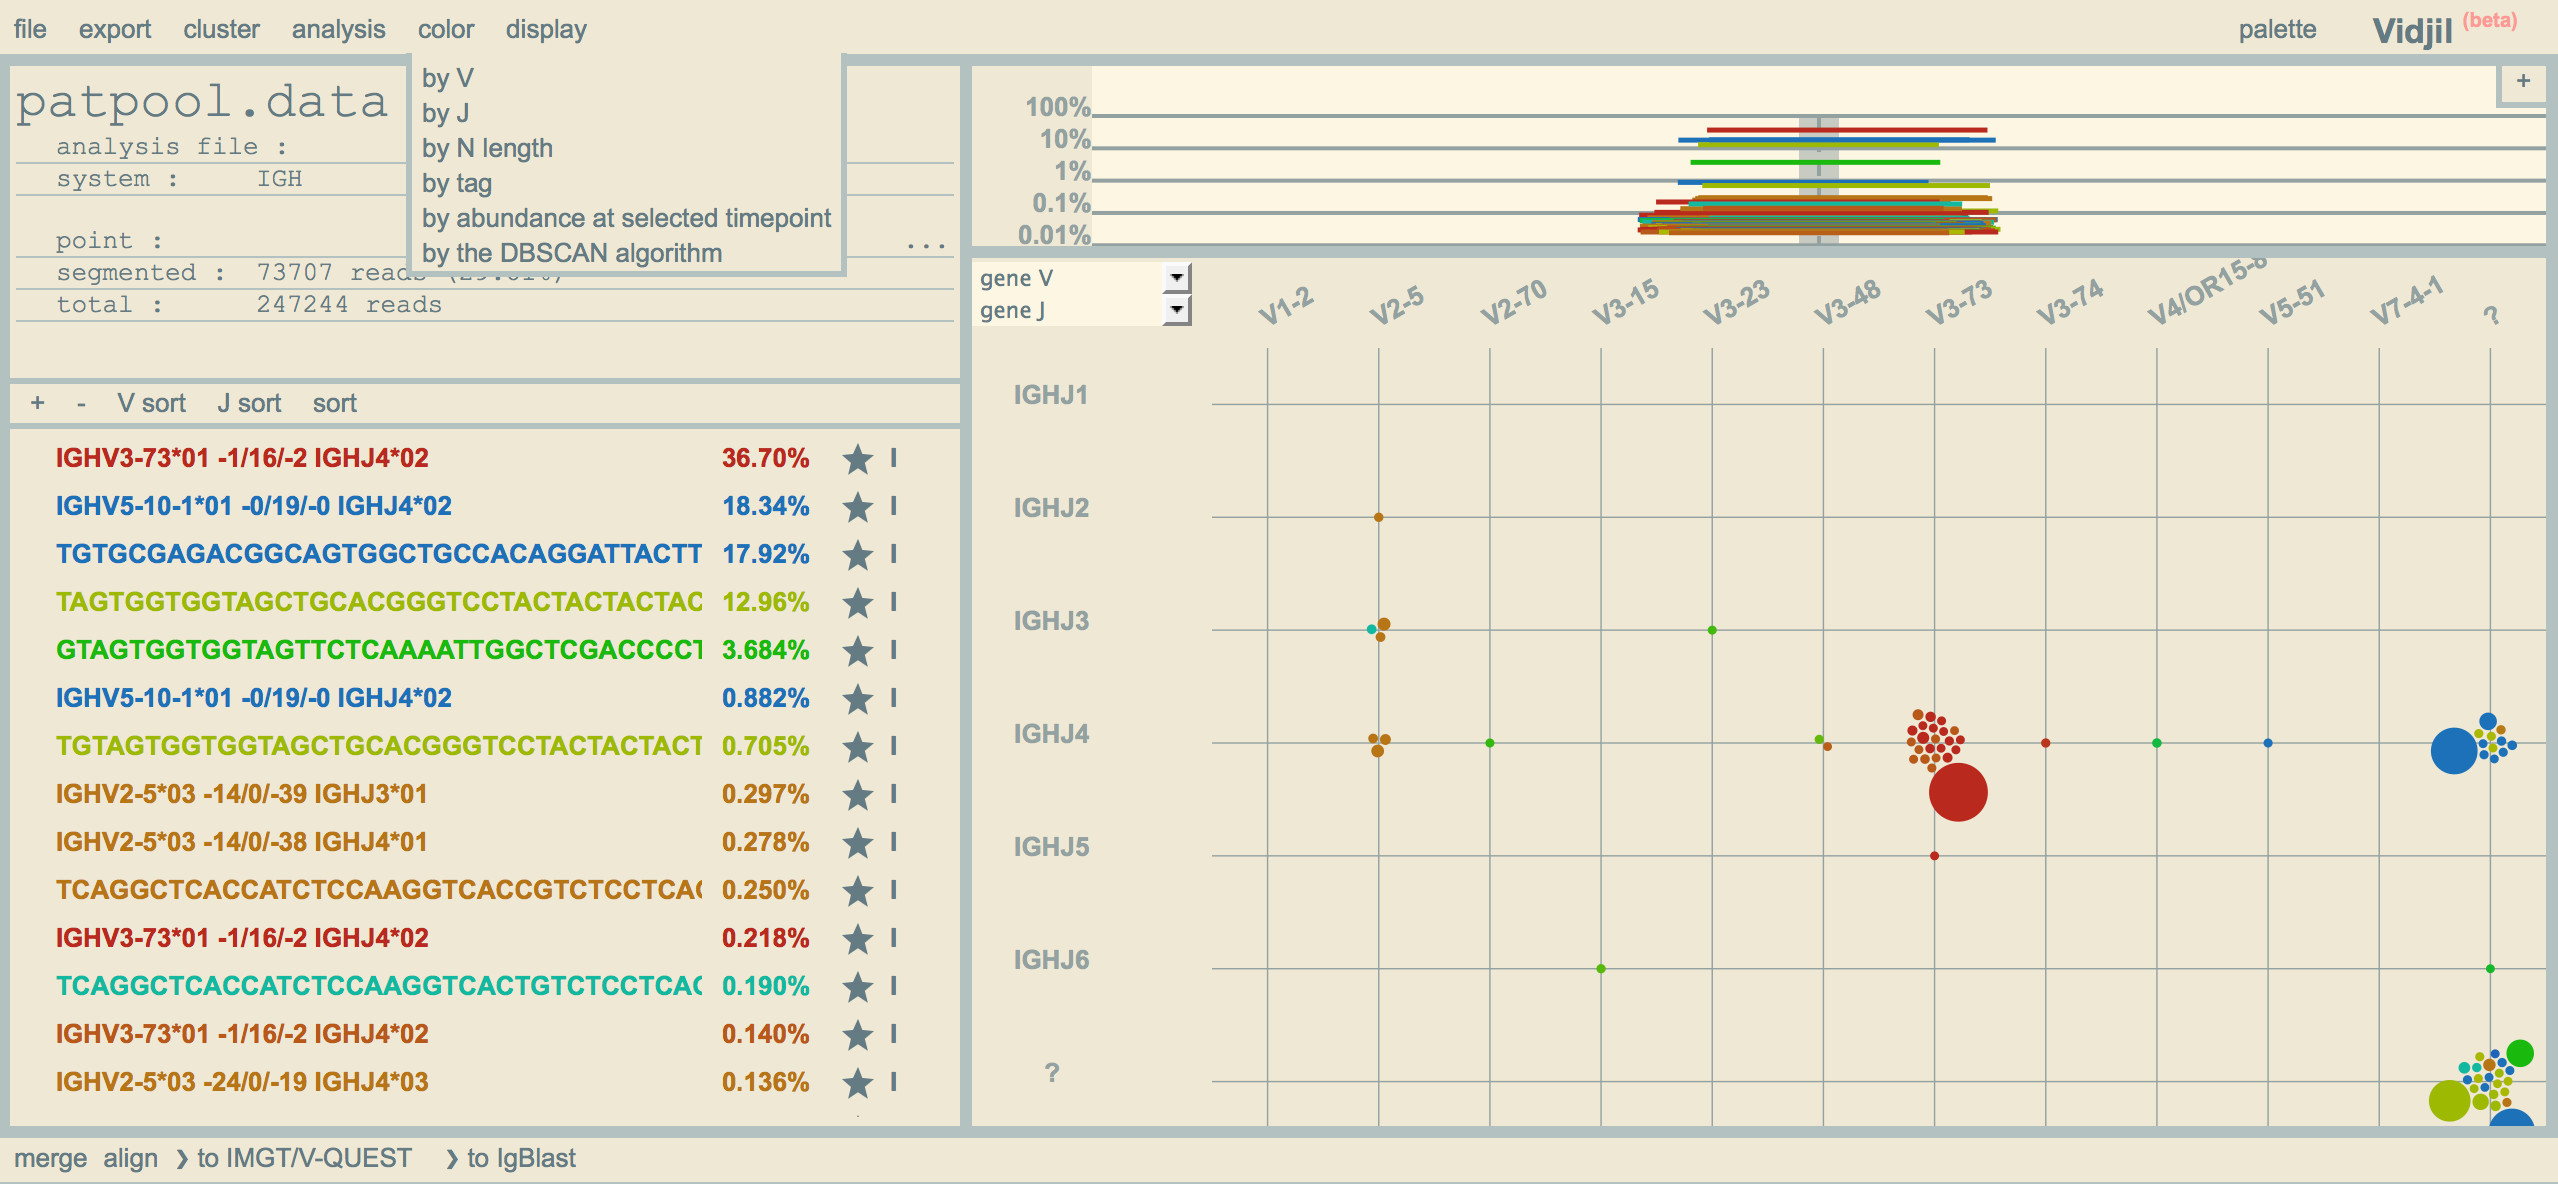
\includegraphics[scale=0.35]{img/DBSCAN-Color-Ex.jpg}
\end{center}
\caption{\textit{Afficheur} avec la colorisation DBSCAN}
\end{figure}

Après cela, j'ai tenté une nouvelle approche en voulant permettre de visualiser dans le \textbf{menu gauche} non pas les clones, mais les clusters issus de DBSCAN.

\begin{figure}[H]
\begin{center}
	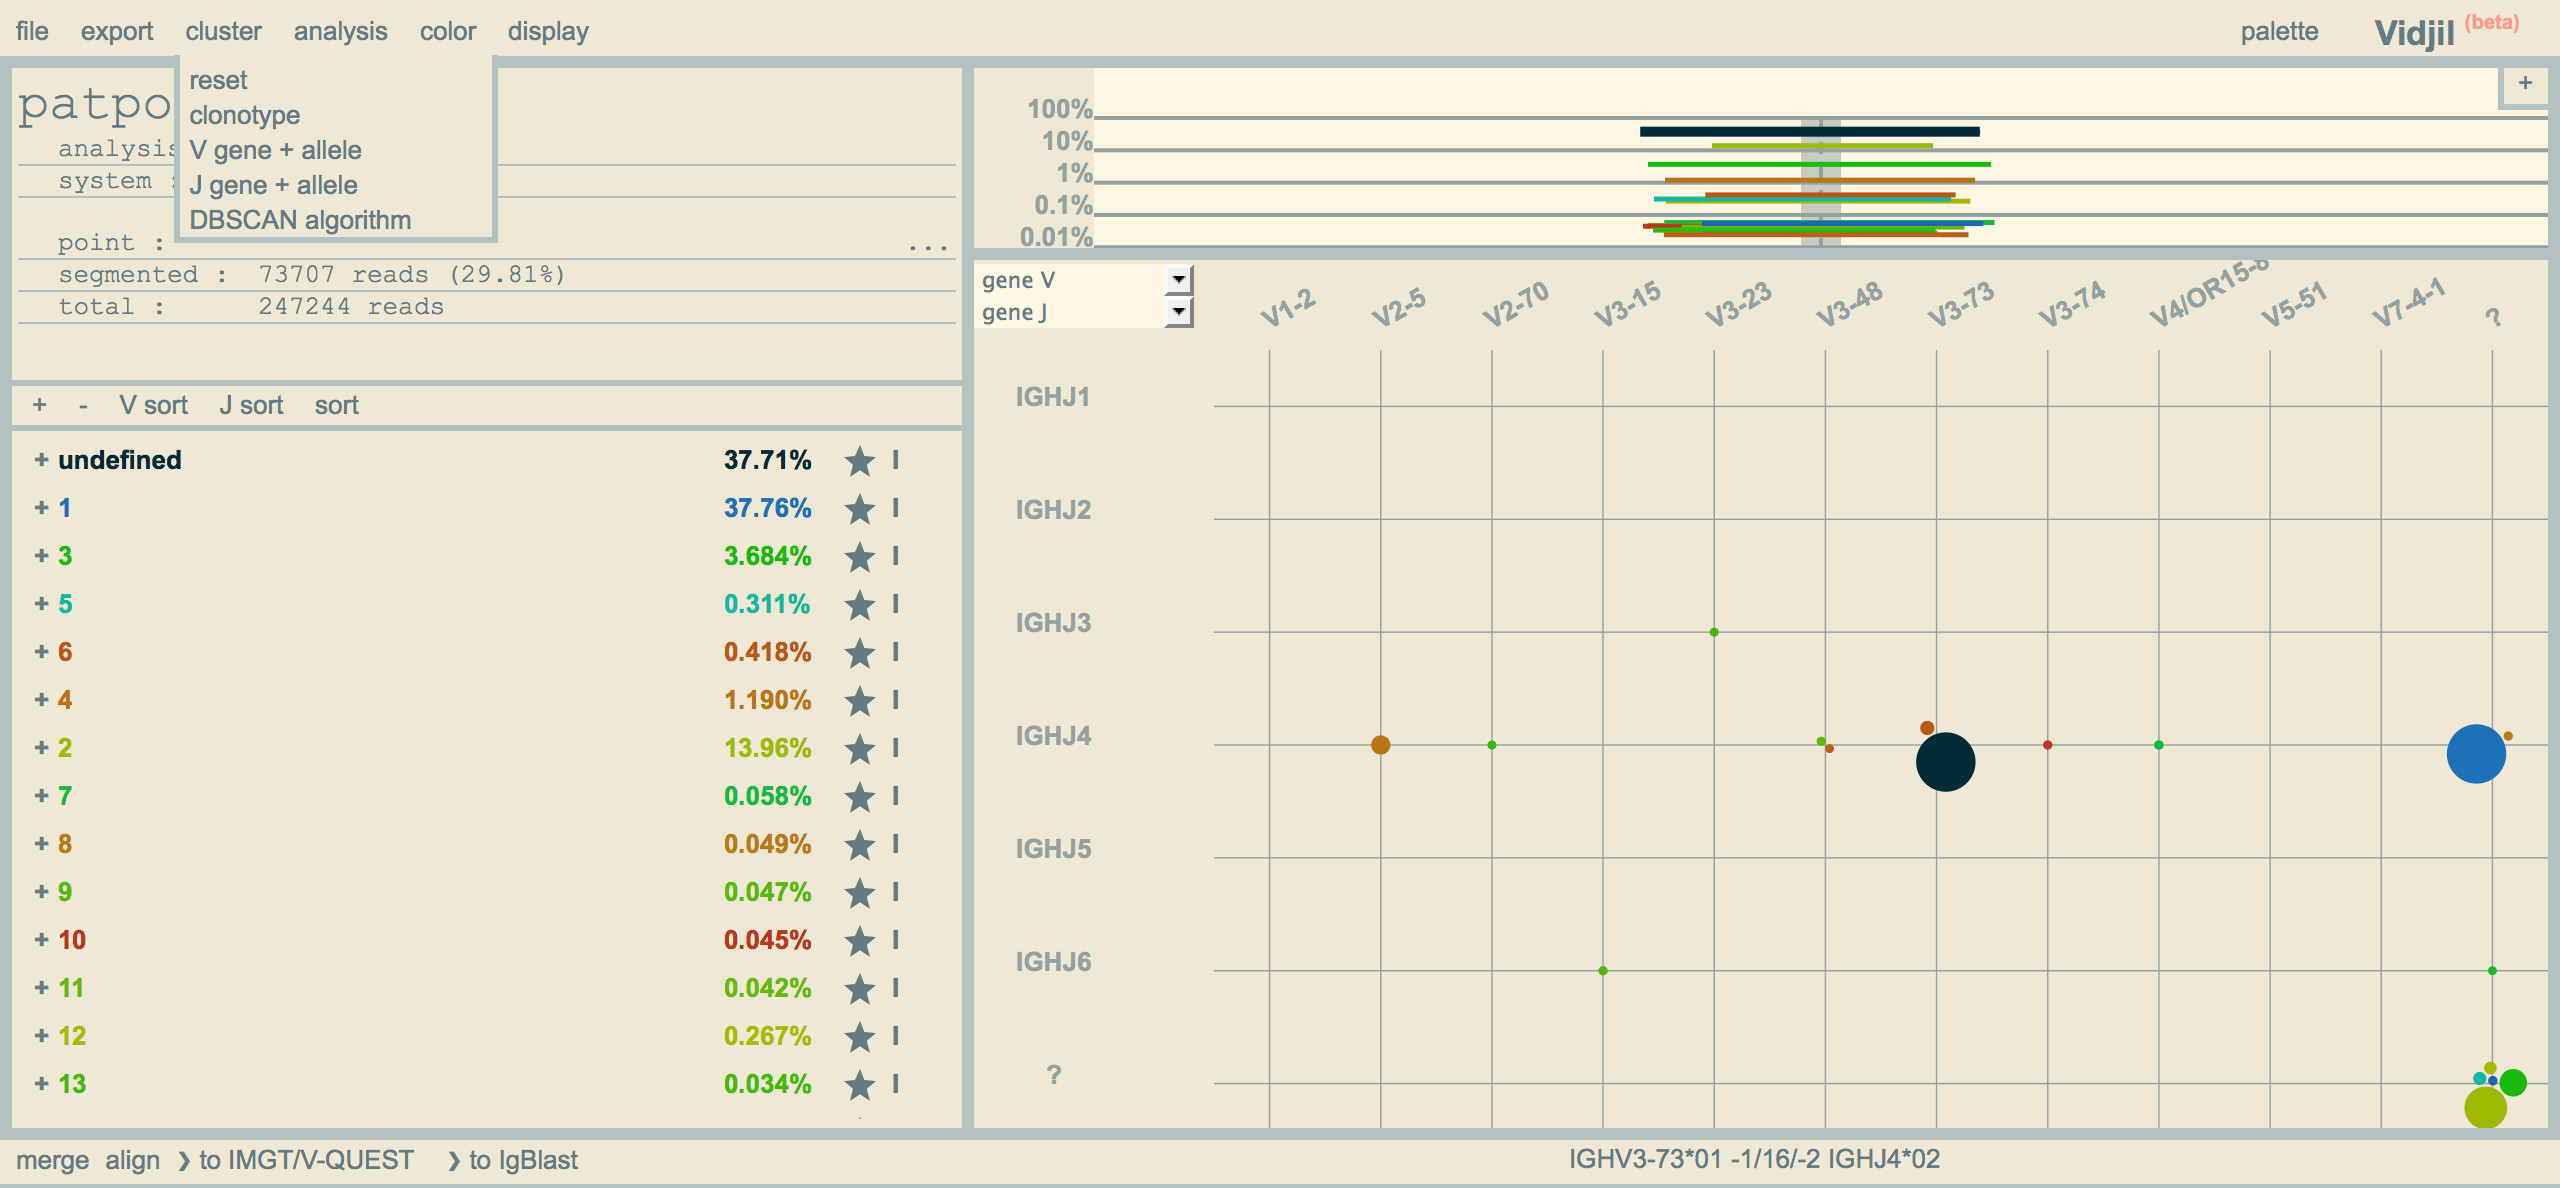
\includegraphics[scale=0.35]{img/DBSCAN-Cluster-Ex.jpg}
\end{center}
\caption{\textit{Afficheur} avec la clusterisation DBSCAN}
\end{figure}

Enfin, en testant plusieurs fois l'algorithme sur des données, je me suis rendu compte qu'il pourrai être bénéfique que les clusters se repoussent mutuellement afin de laisser un maximum de liberté à l'utilisateur, et non pas l'inciter à bouger par lui-même les clusters si les clones issus de ceux-ci sont mélangés, mais aussi que les points \textbf{points centraux} soient au centre de ceux-ci.

\section{Résultats}

L'implémentation de cet algorithme est un vrai succès. En effet, comme nous pouvons le voir sur la figure suivante, la distribution restitue bien une visualisation respectueuse du partitionnement effectué en fonction des données, et des deux paramètres précédemment évoqués.
Cette seconde partie appartient bien à la visualisation intéractive des clones, et est aussi une suite au graphe des distances d'édition, car elle utilise elle aussi ces distances pour fournir un résultat.
Aussi, cette distribution permet d'affirmer que la représentation d'un système permettant de visualiser les similarités et différences entre clones V(D)J est bien mieux respectée par l'implantation de plusieurs graphes distincts, présents dans une seule fenêtre \textit{SVG}.

\begin{figure}[h!]
\begin{center}
	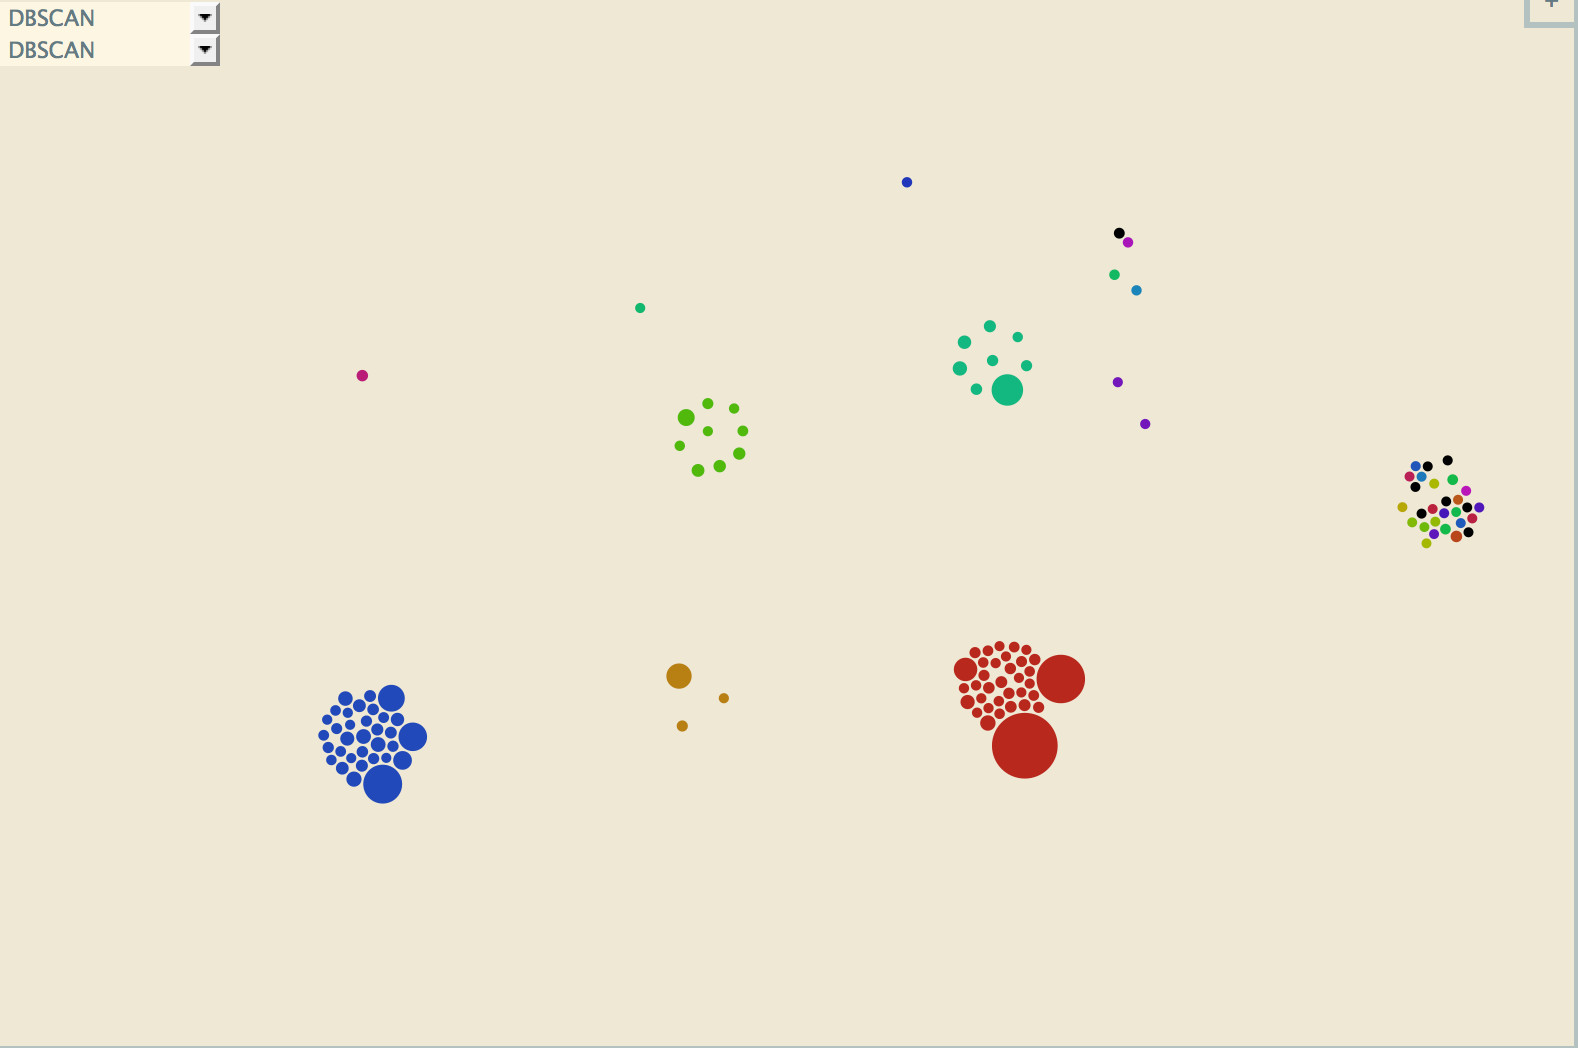
\includegraphics[scale=0.57]{img/DBSCAN-Ex.jpg}
\end{center}
\caption{\textit{Afficheur} avec la distribution DBSCAN}
\end{figure}

\chapter{Recherche et calcul des distances d'édition}

Les distances d'édition sont essentielles quant à la résolution de ma problématique. Ce sont elles qui régissent la structure globale des graphes, et ce sont aussi les principales données des deux distributions que j'ai intégré au projet.
\newline
Auparavant, nous utilisions comme distances des pourcentages d'identité, correspondants à une différence entre deux séquences représentatives appartenant à deux clones quelconques (calculé dans le programme C++) - grosse approximation basée sur des séquences de nucléotides de différentes tailles, et fabriquées à partir des séquences V(D)J et de la \textit{window}. Cette approximation n'étant pas des plus respectables quant à tout le travail précédemment effectué, il a donc fallu obtenir des distances d'édition beaucoup plus précise. J'ai eu alors l'idée de comparer les \textit{windows} de chaque clone V(D)J dans le programme C++, et de retourner le résultat dans le fichier JSON qu'il fournit en sortie.

\section{Utilisation des \textit{windows}}

\subsection{Qu'est-ce qu'une \textit{window}}

Les \textit{windows} sont des séquences suivies de 40 nucléotides, trouvées directement entre la fin de la région V, et le début de la région J après le séquençage. Ces séquences ont été alignées de façon global\footnote{Alignement global: alignement entre deux séquences sur toute leur longueur.}, et non pas en local\footnote{Alignement local: alignement entre une séquence et une partie de l'autre séquence}, comme étaient calculées les pourcentages d'identité.
\newline
\underline{\textbf{Remarque}}: Il se peut donc tout à fait que la partie D se retrouve, ou non, dans cette séquence.

\subsection{Pourquoi les utiliser ?}

L'avantage d'une \textit{window} est qu'elle servira, tout au cours du temps, à marquer spécifiquement un et un seul clone. L'on pourra ainsi faire le suivi de la L.A.L. via l'étude des \textit{windows}, spécifiant des zones bien spécifiques pouvant être contraintes à évoluer en fonction des mutations infligées, ce qui n'était pas possible avec les séquences représentatives.

\begin{figure}[H]
\begin{center}
	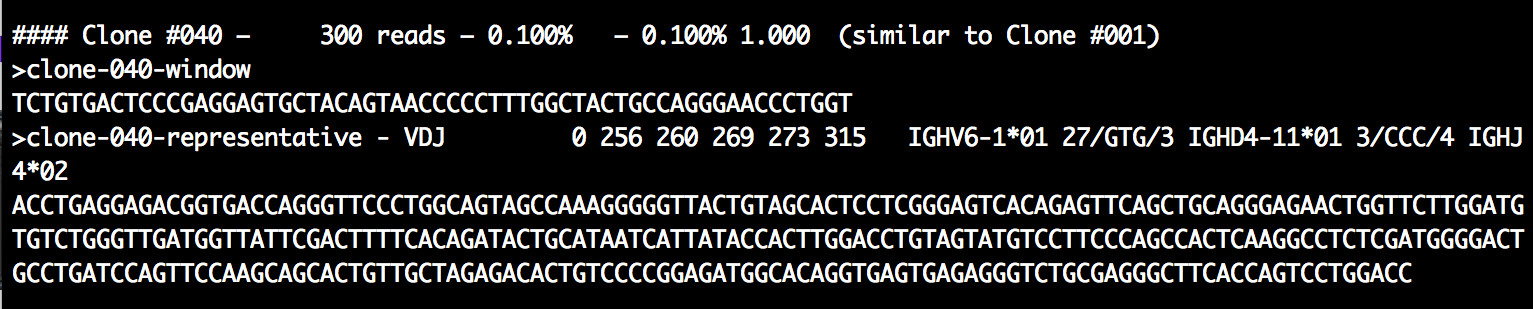
\includegraphics[scale=0.6]{img/C++-window.jpg}
\end{center}
\caption{La \textit{window} du 40ème clone, dans le programme C++, est ici représentée par 'clone-040-window}
\end{figure}

\section{Les différents coûts utilisés}

Les distances d'édition sont calculées grâce à la programmation dynamique\footnote{La Programmation Dynamique est une technique algorithmique pour optimiser des sommes de fonctions monotones croissantes sous contrainte.}, ce qui nous permettra d'obtenir, pour deux mots \textit{x} et \textit{y}, le nombre minimal d’opérations d’édition\footnote{Il y a 3 opérations possibles: la \textbf{substitution} (le remplacement d'une lettre par une autre - nous utiliseront aussi le mot \textit{mismatch} pour cette opération), l'\textbf{insertion} (l'ajout d'une nouvelle lettre), et la \textbf{délétion} (la suppression d'une lettre)} pour transformer \textit{x} en \textit{y} - ce nombre minimal étant la distance d'édition recherchée.

\subsection{Les coûts étudiés}

\subsubsection{Sur quoi est basé un coût?}

Chaque calcul effectué se fait sur un coût, constitué de 5 opérations:
\begin{itemize}
\item{le \textit{match}: la lettre de la séquence 1 sur la position actuelle correspond bien à celle de la séquence 2,}
\item{le \textit{mismatch} (ou substitution): la lettre de la séquence 1 sur la position actuelle ne correspond pas à celle de la séquence 2,}
\item{l'insertion,}
\item{la délétion,}
\item{la détection d'un homopolymère: motif de répétition, le plus souvent attribué par une erreur dans le séquenceur.}
\end{itemize}

\subsubsection{Quels sont ces coûts?}

Pour ces opérations est attribué un poids (n'importe quel entier positif, négatif ou nul), permettant de régir et de calculer une distance, spécifique en fonction de ce poids.
\newline
Ainsi, deux coûts ayant des poids sur ces opérations différentes ne devraient pouvoir obtenir le même résultat (qui sera une distance) à la fin du calcul.
\newline
Il est important de calculer de bons coûts, car ils influeront directement sur les distributions précédemment mises en place. Nous en avons donc sélectionner 4:
\begin{itemize}
\item{le coût de \textbf{\textit{Levenshtein}}: (0, -1, -1): 0 en \textit{match}, -1 en \textit{mismatch}, et -1 en insertion et délétion - la détection d'homopolymère(s) est considéré comme "gratuit" ici, donc ne pèse rien,}
\item{le coût \textbf{\textit{DNA}}: (+5, -4, -10): 5 en \textit{match}, -4 en \textit{mismatch}, et -10 en insertion et délétion - la détection d'homopolymère(s) est aussi considéré comme "gratuit",}
\item{le coût \textbf{\textit{VDJ}}: (+4, -6, -10, -1, -2): 4 en \textit{match}, -6 en \textit{mismatch}, -10 en insertion et délétion, -1 pour les délétions de fin de séquence\footnote{Imaginons que, pour un alignement de deux séquences de longueurs différentes, si la partie de l'une est beaucoup plus grande que l'autre, nous pouvons compter une délétion sur la partie grande (et non-alignée) avec un poids différent.}, -2 pour la détection d'homopolymère(s),}
\item{le coût \textbf{\textit{Identity}}: (+1, -1, -1, 0, 0): 1 en \textit{match}, -1 en \textit{mismatch}, -1 en insertion et délétion, rien pour la détection d'homopolymère(s).}
\end{itemize}
Sur ces 4 coûts, il a fallu choisir celui ayant les plus respectueuses distances par rapport aux similarités entre séquences, afin de perfectionner les distributions.

\begin{table}[H]
\centering
\begin{tabular}{ccccccccc}
   & \textbf{G} & \textbf{A} & \textbf{C} & \textbf{G} & \textbf{A} & \textbf{T} & \textbf{T} & \textbf{A} \\
\textbf{G} & \textbf{0} & -1 & -1 & 0 & -1 & -1 & -1 & -1 \\
\textbf{A} & -1 & \textbf{0} & -1 & -2 & 0 & -1 & -2 & -1 \\
\textbf{T} & -1 & \textbf{-1} & -1 & -2 & -1 & 0 & 0 & -1 \\
\textbf{C} & -1 & -2 & \textbf{-1} & -2 & -2 & -1 & -1 & -1 \\
\textbf{G} & 0 & -2 & -2 & \textbf{-1} & -2 & -2 & -2 & -2 \\
\textbf{A} & -1 & 0 & -1 & -2 & \textbf{-1} & -2 & -3 & -2 \\
\textbf{T} & -1 & -1 & -1 & -2 & -2 & \textbf{-1} & -1 & -2 \\
\textbf{T} & -1 & -2 & -2 & -2 & -3 & -1 & \textbf{-1} & \textbf{\ovalbox{-2}} \\
\end{tabular}
\caption{Calcul de distance d'édition entre 2 séquences ADN (avec \textbf{\textit{Levenshtein}}). 
\newline La distance est entourée - alignement GA\_CGATTA et GATCGATT\_ (le chemin permettant de trouver ces résultats est marqué en \textbf{gras})}
\end{table}

\subsubsection{Comment effectuer les calculs de coût?}

Les coûts étaient déjà implantés à mon arrivée dans l'entreprise, et le programme en C++ contenait déjà un objet (DynProg) prenant en paramètre les deux séquences ADN, l'alignement ainsi que le coût utilisé lors du calcul, et nous renvoyant une matrice de similarité que j'ai transformé en matrice de distances.
\newline
Ainsi, pour étudier les objets \textit{windows} entre eux, il a juste fallu modifier l'alignement local (pris par défaut) par l'alignement global, et le coût par un de notre choix - étant à tester. La matrice est à calculer ou non, en fonction du poids choisi lors du calcul dans la programmation dynamique.

\section{Conclusion}

Les coûts \textit{VDJ}, \textit{Identity} et \textit{Levenshtein} sont les plus probants pour les graphes implémentés. En effet, ce sont eux qui, lors des tests, permettent d'avoir des distances aussi variées que respectueuses des similarités entre clones - ce qui a été vérifié avec un objet Javascript "Stats" (voir \textbf{Figure 16}), implanté directement dans le \textit{scatterplot} en mode \textit{console}, permettant d'obtenir des statistiques sur les arêtes enregistrées par cette vue (comme la moyenne, la distribution ou la médiane par exemple).
\newline
Dû à sa grande popularité, mon choix du coût pour le calcul des distances d'édition entre les \textit{windows} s'est porté vers le coût \textit{Levenshtein}, nous permettant aussi d'obtenir directement des distances d'édition lors du calcul, après les avoir transformé en valeur absolue.

\begin{figure}[H]
\begin{center}
	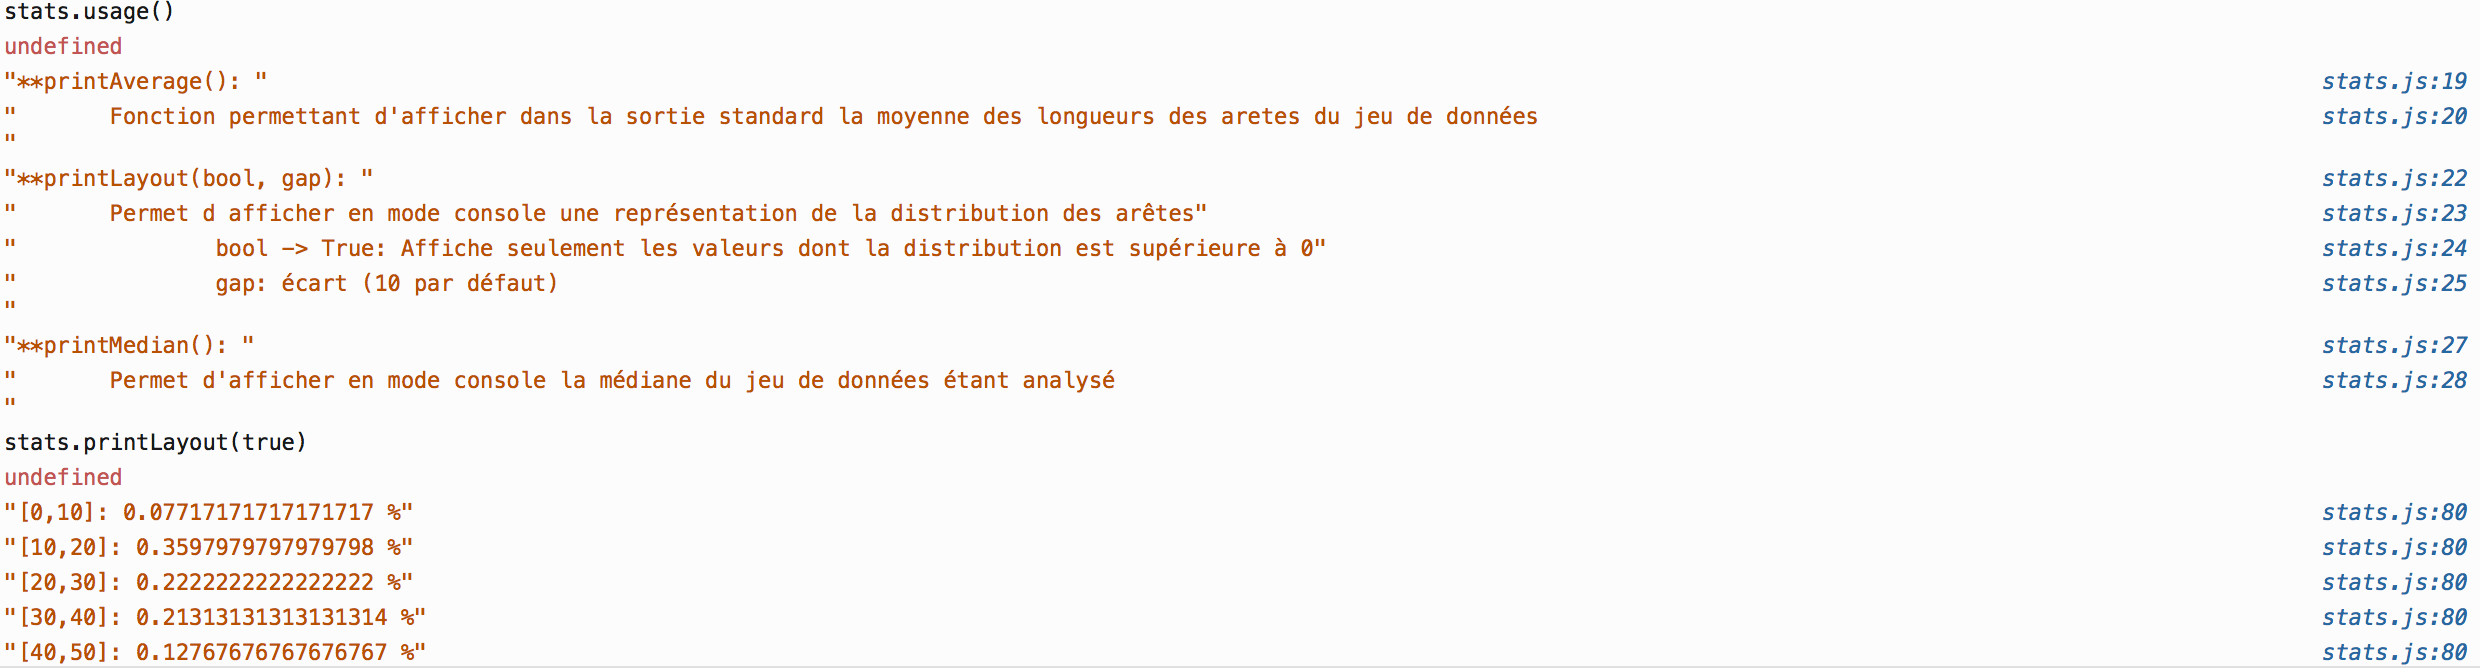
\includegraphics[scale=0.6]{img/Stats.jpg}
\end{center}
\caption{Aperçu de l'objet "Stats", sur un jeu de données avec les distances d'édition de \textit{Levenshtein}}
\end{figure}

\chapter{Le travail en recherche}

Je voulais effectuer mon premier stage Universitaire dans une structure de recherche, étant motivé par l'idée de participer aux solutions et innovations de demain. Ayant effectué un DEUST de Biologie avant de postuler pour une licence d'Informatique à l'Université de Lille1, et étant toujours intéressé par ce domaine de la Science, j'étais très curieux et intéressé de pouvoir effectuer mes premiers pas dans une équipe de bio-informaticiens

\section{La vie est un long fleuve tranquille...}

Mon stage dans l'équipe de recherche \textit{Bonsai} a été un véritable plaisir.
\newline
Eternel curieux, je suis à la recherche perpétuelle d'informations de tous genres pouvant me permettre de progresser dans la vie, mais aussi de m'instruire et me cultiver. L'intérêt et la curiosité de chaque membre de l'équipe envers la Science (à proprement parlé) est imparable, chacun ayant une certaine spécificité en fonction de son parcours et ses intérêts, et qui en fait quelqu'un d'unique dans l'équipe, lui permettant d'échanger avec ses collègues sur ses intérêts dans sa recherche de résultats ou ceux des autres.
\newline
J'ai pu ressentir celà par:
\begin{itemize}
\item \textbf{les conférences/séminaires du Mardi matin}
	\newline
	Chaque mardi matin, généralement entre 11H et 12H, était programmé un séminaire sur un sujet déterminé par le conférencier: un membre de l'équipe \textit{Bonsai} ou un intervenant extérieur.
	\newline
	Nous avons donc pu avoir le plaisir de recevoir des chercheurs de Pennsylvanie et d'un autre État de l'Amérique Centrale, venus nous parler de nouvelles méthodes de recherche, d'attrait à celle-ci, ou des dernières innovations et recherches effectuées sur le sujet donné (\textit{the International Mouse Phenotyping Consortium}\footnote{Entreprise Internationale scientifique créant et caractérisant le phénotype de 20 000 \textit{knock-out} (ou "invalidation génétique" en Français) chez la souris}, les graphes de Bruijn\footnote{Graphe orienté qui permet de représenter les chevauchements de longueur (\textit{n}-1) entre tous les mots de longueur \textit{n} sur un alphabet donné - nom donné par le mathématicien les ayant décrit en 1946: Nicolaas Govert de Bruijn} ou encore la détection des variants complexes \footnote{Variants cytogénétiques constituant une majeure partie des cas de Leucémie myéloïde chronique}) -  mais pas seulement!
	\newline
	Cela a aussi permis à certains membres de l'équipe de pouvoir exposer ses travaux finis ou en cours, afin de pouvoir expliquer son cheminement, sa méthode de travail et ses résultats, comme par exemple le travail d'\textbf{Amandine Perrin} sur l' "Illustration dynamique des effets des vaccins et de la vaccination"\footnote{Travail réalisé entre Mars et Août 2013}.
\item \textbf{les entraides perpétuelles}
	\newline
	Chaque membre de l'équipe peut compter sur les autres s'il a un problème - en effet, l'entraide est omniprésente dans l'équipe, que ce soit pour une aide informatique, algorithmique ou encore de compréhension biologique. Un bref exemple à donner serai celui m'ayant permis de rassembler plus de 5 algorithmes différents, de 5 personnes différentes, pour mon problème de représentation respectueuse d'un graphe à 1000 arêtes.
\item \textbf{la pause déjeuner}
	\newline
	Lors de la pause déjeuner, l'heure est à la discussion scientifique la plupart du temps, et les débats font rage, chacun exposant sa thèse, annonçant et dénonçant un ou plusieurs argument(s) contraire(s) à sa propre vision, etc...
\end{itemize}
Tout ceci m'a permis de me créer une belle idée de ce qu'est le monde de la recherche sur le plan relationnel et scientifique, et de me sentir beaucoup plus à l'aise dès la première semaine de stage.

\section{...ou pas!}

Ce stage m'a permis aussi de me rendre compte de tous les problèmes liés à la recherche, que ce soit pour l'accréditation des sujets de recherche, les problèmes liés aux actions en dehors de sa thèse (le temps attribué à l'éducation, ou encore aux services rendus à l'Université par exemple), ou encore plus directement aux problèmes touchant à son sujet de thèse (la publication du sujet en est un exemple valable).
\newline
Je me suis rendu compte qu'un travail de recherche représentait des heures incalculables à rechercher, programmer, analyser et rédiger - il faut en moyenne entre 6 mois et 1 an (si tout se passe correctement) pour arriver à des résultats valant la peine de les publier.

La problèmatique de la thèse mérite un temps considérablement long à être développée, approfondie et traitée, afin de pouvoir enfin réellement commencer à effectuer ses propres recherches - un peu plus longtemps qu'un nouveau sujet de recherche en général, avec l'expérience, les compétences et la culture en plus.
\newline
Tout ceci est lié à un rythme de publication assez rapide et drastique, qui ne permet pas réellement aux chercheurs de pouvoir travailler dans de bonnes conditions.

La vigilance est aussi de mise quant à la publication des recherches de scientifiques, sur un sujet similaire de celui sur lequel la personne travaille. En effet, un article paraissant à une période très proche d'un autre traitant du même sujet, mais déjà publié, pourrait être refusé en publication pour ce motif.

\chapter*{Conclusion}

\addcontentsline{toc}{chapter}{Conclusion}

\section*{Conclusion par rapport aux objectifs du stage}

Pour les objectifs qui m'ont été donnés en début de stage, le travail sur le graphe de distances d'édition est toujours en cours. Concernant celui-ci, nous ne pouvions pas savoir si le moteur allait réagir correctement par rapport à des distances précises, mon stage étant un test par rapport à son implémentation. Ainsi, il serai préférable de penser au graphe de distances d'édition comme un arbre phylogénétique, ou comme un ensemble de plusieurs graphes comme la distribution DBSCAN. Quant à cette dernière, son implantation a été réalisé avec succès, et démontre bien les ressemblances et disparités entre les clones V(D)J séquencés.

\section*{Conclusion technique}

J'ai beaucoup appris durant ce stage, notamment quant à la conception logicielle - ayant fait de l'ingénierie logicielle durant plusieurs semaines. C'est ce qui m'a appris à travailler en groupe (le respect du travail de mes collègues, les réunions à prévoir, les dead-lines à respecter, le travail logiciel en groupe via l'utilitaire \textit{Git}), à me confronter à un projet déjà existant et pouvoir rentrer au coeur du sujet rapidement, la programmation informatique, l'apprentissage de langages (C++, Python) et de \textit{frameworks} (D3JS, JQuery) informatiques, ainsi que confronter mes idées avec celles des autres et optimiser au possible mon travail, s'il y a nécessité. De plus, ce stage m'a beaucoup apporté en organisation, et j'ai pu confronter le milieu scolaire et le milieu professionnel.

\section*{Conclusion par rapport à la Recherche}

Ce stage a été un avant-goût de ce que va m'apporter le travail dans le milieu de la recherche, ce qui m'a bien conforté dans l'idée de poursuivre mon chemin dans ce monde fabuleux, composé par le travail, la réflexion et l'échange.

\chapter*{Bibliographie - Webographie}

\addcontentsline{toc}{chapter}{Bibliographie - Webographie} 

\begin{itemize}
\item{Le premier article sur le projet \textit{Vidjil}, écrit par M. \textbf{Giraud Mathieu} et M. \textbf{Salson Mikaël}: \url{http://www.biomedcentral.com/1471-2164/15/409/abstract} \textit{(Consultation le 04 Avril 2014)}}
\item{\url{http://www.worldcat.org/title/recombinaison-vdj-illegitime-et-developpement-de-leucemies-aigues-lymphoblastiques-t/oclc/495056914} \textit{(Consultation le 10 Mai 2014)}}
\item{\url{http://fr.wikipedia.org/wiki/Recombinaison_V%28D%29J} \textit{(Consultation le 10 Mai 2014)}}
\item{\url{http://fr.wikipedia.org/wiki/DBSCAN} \textit{(Consultation le 19 Mai 2014)}}
\item{\url{http://citeseerx.ist.psu.edu/viewdoc/download?doi=10.1.1.88.4045&rep=rep1&type=pdf} \textit{(Consultation le 19 Mai 2014)}}
\item{\url{http://www.cise.ufl.edu/class/cis4930sp09dm/notes/dm5part4.pdf} \textit{(Consultation le 19 Mai 2014)}}
\end{itemize}


\end{spacing}
\end{document}